% !TEX program = xelatex
% Biên dịch: xelatex main.tex (chạy 2 lần để cập nhật mục lục & tham chiếu)
\RequirePackage{fix-cm}
\documentclass[a4paper]{article}

% ---------- Cỡ chữ 13pt thật sự (lớp report chuẩn chỉ hỗ trợ 10/11/12pt,
% nên option [13pt] bị bỏ qua; gói fontsize cho phép đặt cỡ tuỳ ý) ----------
\usepackage[fontsize=13pt]{fontsize}

% ---------- Ngôn ngữ & font (XeLaTeX) ----------
\usepackage{fontspec}
\usepackage{amsmath}
\usepackage{unicode-math}
\usepackage{polyglossia}
\setdefaultlanguage{vietnamese}
% Font Latin Modern (font TeX cổ điển) — giống bài mẫu, có hỗ trợ tiếng Việt
\setmainfont{Latin Modern Roman}
\setmathfont{Latin Modern Math}
% LM Mono không có bản bold → ánh xạ bold về regular để tránh cảnh báo font
\setmonofont{Latin Modern Mono}[BoldFont={Latin Modern Mono}]

% ---------- Trình bày trang ----------
\usepackage[a4paper,left=3.5cm,right=2cm,top=2.5cm,bottom=2.5cm]{geometry}
\usepackage{setspace}
\onehalfspacing
% Cho phép TeX nới dòng ở bước cuối để tránh text tràn lề (overfull hbox)
\setlength{\emergencystretch}{3em}
% Bỏ qua các cảnh báo underfull nhẹ do tiếng Việt và tên vùng dài trong danh sách.
\hbadness=2000

% ---------- Hình, bảng, biểu ----------
\usepackage{graphicx}
\graphicspath{{figures/}}
\usepackage{float}
\usepackage{booktabs}
\usepackage{longtable}
\usepackage{array}
\usepackage{multirow}
\usepackage{makecell}
\usepackage[font=small,labelfont=bf]{caption}
\usepackage{subcaption}
\usepackage[table]{xcolor}

% ---------- Liên kết ----------
\usepackage[hidelinks]{hyperref}
\usepackage{enumitem}

% \code: định danh dạng monospace; cho phép ngắt dòng ngay sau dấu gạch dưới
% để các tên biến dài (vd. num_of_prev_attempts) không tràn ra lề.
\newcommand{\code}[1]{{\ttfamily\def\_{\textunderscore\discretionary{}{}{}}#1}}
\pdfstringdefDisableCommands{%
  \def\code#1{#1}%
  \def\_{ }%
}

\begin{document}

% =====================================================================
%  TRANG BÌA
% =====================================================================
\begin{titlepage}
  \centering
  {\large\bfseries TRƯỜNG ĐẠI HỌC QUY NHƠN\\[3pt]
   KHOA TOÁN \& THỐNG KÊ\par}

  \vspace{1.3cm}

  % ----- LOGO trường -----
  
\includegraphics[width=3.5cm]{logo_qnu.png}\par

  \vspace{1.4cm}

  {\bfseries TIỂU LUẬN MÔN HỌC:\\[3pt]
   PHÂN TÍCH DỮ LIỆU KHOA HỌC CHUYÊN NGÀNH\par}

  \vspace{0.5cm}
  \rule{\textwidth}{0.4pt}\\[0.55cm]
  {\LARGE\bfseries XÂY DỰNG VÀ SO SÁNH MÔ HÌNH\\[6pt]
   HỌC MÁY CẢNH BÁO SỚM\\[6pt]
   RỦI RO HỌC TẬP\par}
  \vspace{0.5cm}
  \rule{\textwidth}{0.4pt}

  \vspace{2.4cm}

  {\normalsize
  \begin{tabular}{r@{\hspace{0.5em}}l}
    \itshape Trình độ đào tạo:      & Thạc sĩ \\[5pt]
    \itshape Học viên thực hiện:    & Nguyễn Hồ Bảo Thiên \\[5pt]
    \itshape Mã số sinh viên:       & 8282548017 \\[5pt]
    \itshape Lớp:                   & Khoa học dữ liệu K28B \\[5pt]
    \itshape Giảng viên hướng dẫn:  & TS. Hồ Văn Lâm \\
  \end{tabular}\par}

  \vfill
  {\itshape Gia Lai, 2026\par}
\end{titlepage}

% =====================================================================
%  PHẦN ĐẦU (mục lục, danh mục hình/bảng) — đánh số La Mã
% =====================================================================
\pagenumbering{roman}
\tableofcontents
\listoffigures
\listoftables
\clearpage

% =====================================================================
%  NỘI DUNG CHÍNH — đánh số Ả Rập
% =====================================================================
\pagenumbering{arabic}

\section{Giới thiệu}

Báo cáo này trình bày giai đoạn \textit{xây dựng và so sánh mô hình học máy}
cho bài toán cảnh báo sớm rủi ro học tập, kế thừa trực tiếp kết quả của giai
đoạn phân tích khám phá dữ liệu (EDA) trước đó. Bài toán được xác định lại ở
dạng \textbf{phân loại nhị phân}: nhận diện sinh viên \textbf{có nguy cơ}
(At-risk) --- gộp từ hai nhóm kết quả trượt môn (Fail) và bỏ học (Withdrawn)
--- so với nhóm \textbf{hoàn thành} (Pass), dựa trên đặc trưng nhân khẩu học và
hành vi học tập tích luỹ đến một mốc thời gian xác định trong khoá học.

Nội dung báo cáo gồm bốn phần chính:

\begin{enumerate}[leftmargin=*]
  \item \textbf{Tiền xử lý dữ liệu}: điền giá trị thiếu, mã hoá đặc trưng phân
        loại, gộp nhãn và chuẩn hoá bài toán về dạng nhị phân.
  \item \textbf{Khảo sát sơ bộ theo các mốc dự đoán}: huấn luyện một mô hình cơ
        sở xuyên suốt toàn bộ các mốc thời gian trong khoá học để hiểu xu hướng
        hiệu suất theo thời gian, làm cơ sở lựa chọn mốc dự đoán cho các thử
        nghiệm chuyên sâu.
  \item \textbf{Xây dựng mô hình}: huấn luyện và tinh chỉnh bốn thuật toán học
        máy (Logistic Regression, Random Forest, CatBoost, LightGBM) kết hợp kỹ
        thuật xử lý mất cân bằng nhãn, tập trung vào mốc thời gian đã chọn.
  \item \textbf{So sánh và diễn giải mô hình}: đối chiếu hiệu suất giữa các
        thuật toán, đánh giá độ ổn định khi rút gọn số lượng đặc trưng, và diễn
        giải các dự báo bằng phương pháp SHAP.
\end{enumerate}

\section{Tiền xử lý dữ liệu}

\subsection{Điền giá trị thiếu ở đặc trưng động}

Các đặc trưng phản ánh hành vi học tập tích luỹ (tương tác với hệ thống học
trực tuyến và kết quả bài đánh giá) có giá trị thiếu ở những sinh viên chưa
từng tương tác hoặc chưa nộp bài nào tính đến mốc thời gian quan sát. Quy tắc
điền khuyết được áp dụng riêng cho từng nhóm đặc trưng:

\begin{itemize}[leftmargin=*]
  \item \textbf{Đặc trưng tương tác VLE} (\code{total\_clicks},
        \code{active\_weeks}, \code{avg\_weekly\_clicks}) và \textbf{đặc trưng
        bài đánh giá} (\code{num\_submitted}, \code{num\_failed}) --- điền bằng
        0, vì giá trị thiếu ở đây đồng nghĩa với việc sinh viên chưa phát sinh
        hoạt động nào.
  \item \code{avg\_score} --- điền bằng giá trị \textbf{-1} (nằm ngoài thang
        điểm $[0, 100]$) để phân biệt rõ ràng với trường hợp sinh viên nộp bài
        và bị điểm 0.
  \item \code{avg\_days\_early} --- điền bằng 0; thông tin về việc sinh viên
        không nộp bài dù đã đến hạn đã được nắm bắt riêng bởi đặc trưng nhị
        phân \code{no\_submission\_despite\_due}, nên việc điền 0 ở đây không
        gây nhầm lẫn.
\end{itemize}

Sau bước điền khuyết, toàn bộ đặc trưng động không còn giá trị thiếu.

\subsection{Xử lý giá trị thiếu ở \code{imd\_band}}

Như đã trình bày ở giai đoạn phân tích khám phá, biến \code{imd\_band} (chỉ số
thiếu thốn kinh tế theo khu vực) có một dạng thiếu riêng biệt, được mã hoá bằng
ký hiệu \code{'?'} thay vì giá trị rỗng thông thường. Một biến chỉ báo
\code{imd\_missing} được tạo trước khi điền khuyết, để mô hình có thể tận dụng
chính tín hiệu ``thiếu dữ liệu'' như một đặc trưng dự báo.

Giá trị thiếu được điền theo \textbf{phân phối riêng của từng vùng}
(\code{region}), ước lượng trên tập huấn luyện rồi áp dụng lại cho tập kiểm
tra. Sau bước xử lý, biến \code{imd\_band\_filled} không còn giá trị thiếu ở
cả hai tập huấn luyện và kiểm tra.

\subsection{Mã hoá đặc trưng phân loại}

Các đặc trưng phân loại được mã hoá theo bản chất của từng biến, tóm tắt ở
Bảng~\ref{tab:encoding}.

\begin{table}[H]
  \centering
  \caption{Phương án mã hoá các đặc trưng phân loại.}
  \label{tab:encoding}
  \begin{tabular}{lll}
    \toprule
    \textbf{Đặc trưng} & \textbf{Kiểu mã hoá} & \textbf{Lý do} \\
    \midrule
    \code{disability}         & Nhị phân & Y $\to$ 1, N $\to$ 0 \\
    \code{highest\_education} & Thứ tự (ordinal) & Có thứ bậc học vấn rõ ràng \\
    \code{imd\_band\_filled}  & Thứ tự (ordinal) & Có thứ bậc mức độ nghèo \\
    \bottomrule
  \end{tabular}
\end{table}

Ba đặc trưng nhân khẩu học còn lại từ dữ liệu gốc --- \code{gender},
\code{region}, \code{age\_band} --- không được đưa vào ma trận đặc trưng huấn
luyện. Các đặc trưng nhân khẩu học được giữ lại (\code{highest\_education},
\code{disability}, \code{imd\_band\_filled}) là những đặc trưng đã cho thấy
liên hệ rõ ràng với kết quả học tập ở giai đoạn phân tích khám phá dữ liệu
trước đó.

\subsection{Tập đặc trưng cuối cùng}

Sau các bước xử lý trên, ma trận đặc trưng dùng cho huấn luyện mô hình gồm
\textbf{15 đặc trưng}:

\begin{itemize}[leftmargin=*]
  \item \textbf{Tĩnh (5):} \code{highest\_education}, \code{disability},
        \code{num\_of\_prev\_attempts}, \code{studied\_credits},
        \code{imd\_band\_filled}, cùng biến chỉ báo \code{imd\_missing}.
  \item \textbf{Động (9):} \code{total\_clicks\_filled},
        \code{active\_weeks\_filled}, \code{avg\_weekly\_clicks\_filled},
        \code{num\_due}, \code{num\_submitted\_filled},
        \code{avg\_score\_filled}, \code{num\_failed\_filled},
        \code{avg\_days\_early\_filled}, \code{no\_submission\_despite\_due}.
\end{itemize}

Việc chia tập huấn luyện và kiểm tra được giữ nguyên theo \textbf{từng sinh
viên} như đã thiết lập ở giai đoạn EDA (tỷ lệ 80:20), đảm bảo không xảy ra rò
rỉ dữ liệu giữa hai tập.

\subsection{Chuẩn hoá bài toán về phân loại nhị phân}

Với mục tiêu cảnh báo sớm, ranh giới quan trọng nhất không nằm giữa Fail và
Withdrawn, mà giữa nhóm \textbf{hoàn thành} và nhóm \textbf{không hoàn thành}
học phần. Do đó, nhãn mục tiêu được chuẩn hoá lại:

\[
  \text{At-risk (1)} = \text{Fail} \cup \text{Withdrawn}, \qquad
  \text{Pass (0)} = \text{Pass}.
\]

Phép gộp nhãn này được áp dụng thống nhất cho toàn bộ dữ liệu dạng panel, tức
trên mọi bản ghi ở cả tám mốc dự đoán $T \in \{30, 60, \ldots, 240\}$ đã thiết
kế ở giai đoạn EDA --- không giới hạn ở một mốc thời gian cụ thể nào. Với dữ
liệu đã ở dạng nhị phân, câu hỏi tiếp theo là mốc dự đoán nào nên được chọn để
huấn luyện và đánh giá mô hình; đây là nội dung được khảo sát ở phần kế tiếp.

\section{Khảo sát sơ bộ theo các mốc dự đoán}
\label{sec:snapshot_survey}

Trước khi đi sâu so sánh nhiều thuật toán tại một mốc thời gian cố định, cần
khảo sát sơ bộ hiệu suất mô hình học máy \textbf{xuyên suốt toàn bộ các mốc dự
đoán} đã thiết kế ở giai đoạn tiền xử lý, nhằm hai mục đích: (i) hiểu xu hướng
biến động hiệu suất theo thời gian khi sinh viên tích luỹ ngày càng nhiều hành
vi học tập, và (ii) làm cơ sở lựa chọn một mốc thời gian đại diện, phù hợp cho
các thử nghiệm chuyên sâu ở phần sau.

\subsection{Thiết lập thử nghiệm}

Với mỗi mốc dự đoán $T$, một mô hình \textbf{Logistic Regression} được huấn
luyện riêng, chỉ sử dụng dữ liệu của đúng mốc đó --- đây cũng là thuật toán cơ
sở, đơn giản và dễ diễn giải nhất trong bốn thuật toán được đề xuất ở giai
đoạn EDA, phù hợp để khảo sát nhanh xu hướng hiệu suất theo thời gian trước
khi mở rộng sang các mô hình phức tạp hơn. Quy trình tinh chỉnh áp dụng cho
từng mô hình tương tự cách tiếp cận sẽ được dùng ở giai đoạn so sánh nhiều
thuật toán tại Mục~\ref{sec:methodology}: dữ liệu được chuẩn hoá bằng
\code{StandardScaler} (fit trên train-fold, tránh rò rỉ dữ liệu), siêu tham số
điều chuẩn $C$ của mô hình, tỷ lệ oversampling SMOTE và trọng số lớp At-risk
được tinh chỉnh đồng thời bằng Optuna (30 lượt thử nghiệm, kiểm định chéo phân
tầng 3-fold), sau đó huấn luyện lại trên toàn bộ tập huấn luyện của mốc đó và
đánh giá trên tập kiểm tra giữ nguyên.

Một lưu ý về mặt phương pháp: ở lần thử đầu tiên, hàm mục tiêu tối ưu là
\textit{recall thuần} của lớp At-risk, nhưng cách làm này khiến mô hình suy
biến về việc dự đoán \textbf{toàn bộ} sinh viên đều là At-risk (recall đạt gần
tuyệt đối nhưng precision rất thấp, không có giá trị thực tiễn). Hàm mục tiêu
sau đó được đổi sang \textbf{F1-score của lớp At-risk} để buộc mô hình cân
bằng giữa precision và recall --- đây là hàm mục tiêu được giữ nguyên xuyên
suốt các thử nghiệm còn lại của báo cáo.

\subsection{Kết quả theo thời gian}

Bảng~\ref{tab:snapshot_results} tổng hợp hiệu suất trên tập kiểm tra của tám
mô hình, mỗi mô hình ứng với một mốc dự đoán.

\begin{table}[H]
  \centering
  \caption{Kết quả sơ bộ của mô hình Logistic Regression --- một mô hình riêng cho mỗi mốc dự đoán $T$ --- trên tập kiểm tra. Precision/Recall/F1 tính riêng cho lớp At-risk.}
  \label{tab:snapshot_results}
  \small
  \begin{tabular}{rrrrrrr}
    \toprule
    \textbf{T (ngày)} & \textbf{Train} & \textbf{Test} & \textbf{Accuracy} & \textbf{Precision} & \textbf{Recall} & \textbf{F1} \\
    \midrule
    30 & 19{,}988 & 5{,}043 & 0.6443 & 0.5698 & 0.8115 & 0.6695 \\
    60 & 19{,}123 & 4{,}835 & 0.7369 & 0.6734 & 0.7258 & 0.6986 \\
    90 & 18{,}508 & 4{,}680 & 0.7402 & 0.6442 & 0.7857 & 0.7080 \\
    120 & 17{,}917 & 4{,}518 & 0.7900 & 0.7096 & 0.7555 & 0.7318 \\
    150 & 17{,}386 & 4{,}363 & 0.8260 & 0.7561 & 0.7575 & 0.7568 \\
    180 & 16{,}786 & 4{,}215 & 0.8458 & 0.7552 & 0.7980 & 0.7760 \\
    210 & 16{,}486 & 4{,}162 & 0.8640 & 0.7960 & 0.7842 & 0.7901 \\
    240 & 16{,}190 & 4{,}094 & 0.8774 & 0.8152 & 0.7899 & \textbf{0.8024} \\
    \bottomrule
  \end{tabular}
\end{table}


Hình~\ref{fig:trend_snapshot} trực quan hoá xu hướng của bốn chỉ số theo mốc
thời gian.

\begin{figure}[H]
  \centering
  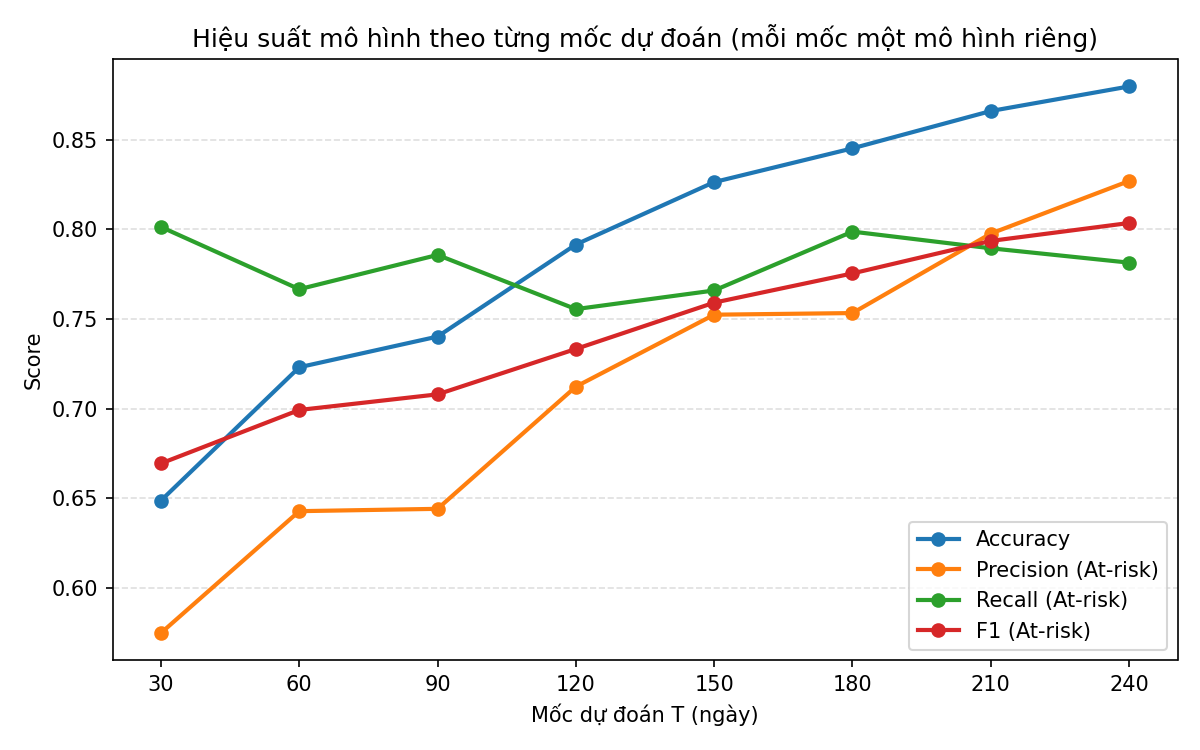
\includegraphics[width=0.85\textwidth]{trend_by_snapshot.png}
  \caption{Xu hướng hiệu suất mô hình theo từng mốc dự đoán (mỗi mốc một mô
  hình riêng).}
  \label{fig:trend_snapshot}
\end{figure}

\begin{itemize}[leftmargin=*]
  \item \textbf{Accuracy} và \textbf{precision At-risk} tăng \textbf{đơn điệu
        tuyệt đối} theo thời gian --- không có mốc nào sụt giảm so với mốc
        liền trước (accuracy từ 0.6488 ở $T=30$ lên 0.8796 ở $T=240$; precision
        từ 0.5750 lên 0.8269) --- phù hợp với trực giác: sinh viên càng tích
        luỹ nhiều hành vi học tập, tín hiệu dự báo càng rõ ràng và đáng tin cậy
        hơn.
  \item \textbf{Recall At-risk} lại dao động trong một biên độ hẹp
        (0.7555--0.8013) mà không theo xu hướng rõ ràng, thậm chí đạt giá trị
        cao nhất ngay ở mốc sớm nhất $T=30$ (0.8013) --- khi độ chính xác tổng
        thể còn rất thấp (accuracy 0.6488, precision 0.5750). Điều này cho
        thấy ở giai đoạn đầu khoá, khi tín hiệu hành vi còn thưa thớt, ranh
        giới tuyến tính của Logistic Regression có xu hướng dự báo At-risk khá
        rộng rãi --- bắt được phần lớn sinh viên có nguy cơ nhưng đánh đổi
        bằng rất nhiều cảnh báo nhầm.
  \item \textbf{F1 At-risk} --- chỉ số tổng hợp được dùng làm mục tiêu tối ưu
        --- vì vậy cũng tăng đơn điệu tuyệt đối theo thời gian, từ 0.6695
        ($T=30$) lên 0.8035 ($T=240$), nhưng động lực tăng chủ yếu đến từ
        \textbf{precision} chứ không phải recall, vốn gần như đi ngang xuyên
        suốt khoá học.
\end{itemize}

Ma trận nhầm lẫn của cả tám mô hình được thể hiện ở Hình~\ref{fig:cm_snapshot}.

\begin{figure}[H]
  \centering
  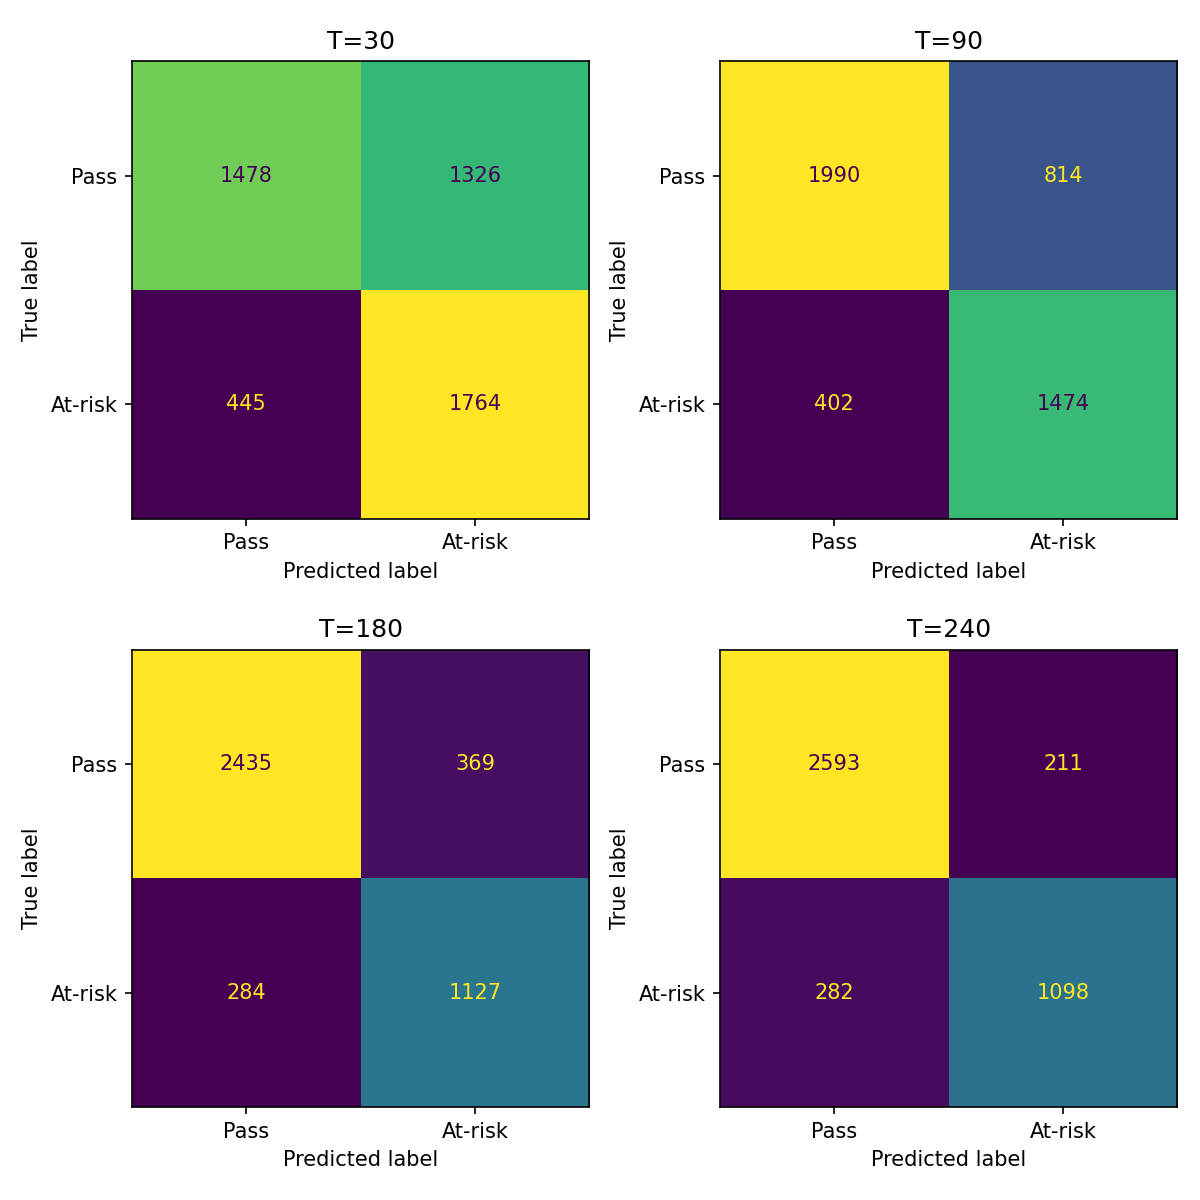
\includegraphics[width=\textwidth]{cm_grid_snapshots.png}
  \caption{Ma trận nhầm lẫn trên tập kiểm tra tại từng mốc dự đoán.}
  \label{fig:cm_snapshot}
\end{figure}

Bảng~\ref{tab:snapshot_params} cho thấy siêu tham số xử lý mất cân bằng nhãn
mà Optuna lựa chọn theo từng mốc thời gian.

\begin{table}[H]
  \centering
  \caption{Siêu tham số xử lý mất cân bằng nhãn được Optuna lựa chọn cho từng mốc dự đoán, cùng F1 At-risk trung bình qua 3-fold cross-validation.}
  \label{tab:snapshot_params}
  \begin{tabular}{rrrr}
    \toprule
    \textbf{T (ngày)} & \textbf{F1 At-risk (CV)} & \textbf{Tỷ lệ SMOTE} & \textbf{Trọng số At-risk} \\
    \midrule
    30 & 0.6723 & +0.56x & 1.24 \\
    60 & 0.7065 & +0.63x & 1.01 \\
    90 & 0.7160 & +0.57x & 1.33 \\
    120 & 0.7485 & +0.53x & 1.13 \\
    150 & 0.7762 & +0.43x & 1.11 \\
    180 & 0.7923 & +0.88x & 1.01 \\
    210 & 0.8042 & +0.51x & 1.03 \\
    240 & 0.8174 & +0.51x & 1.03 \\
    \bottomrule
  \end{tabular}
\end{table}


Trọng số At-risk tối ưu hầu như luôn hội tụ gần giá trị 1 (1.01--1.33) ở mọi
mốc thời gian, trong khi tỷ lệ SMOTE dao động ở mức khá cao và không theo xu
hướng rõ rệt (0.42--0.90x). Nói cách khác, với Logistic Regression, việc bổ
sung mẫu tổng hợp qua SMOTE đóng vai trò chủ đạo trong xử lý mất cân bằng
nhãn, hơn là điều chỉnh trọng số lớp --- đây là đặc điểm nhất quán của thuật
toán này, cũng sẽ được quan sát lại khi so sánh với ba thuật toán còn lại ở
Bảng~\ref{tab:best_params}.

\subsection{Lựa chọn mốc dự đoán cho phân tích chuyên sâu}
\label{sec:choose_t150}

Kết quả khảo sát cho thấy một sự đánh đổi rõ ràng giữa \textbf{độ tin cậy của
dự báo} và \textbf{thời gian còn lại để can thiệp}: các mốc càng muộn cho hiệu
suất càng cao, nhưng đồng thời càng gần thời điểm kết thúc khoá học, làm giảm
giá trị thực tiễn của một cảnh báo sớm. Với khoá học OULAD kéo dài khoảng
240--270 ngày, hai mốc cho F1 cao nhất --- 210 và 240 ngày, lần lượt 0.7935 và
0.8035 --- chỉ còn lại khoảng 10--20\% thời lượng khoá học, quá muộn để nhà
trường triển khai các biện pháp hỗ trợ có ý nghĩa.

Mốc \textbf{150 ngày} được chọn làm đại diện cho các thử nghiệm chuyên sâu ở
phần còn lại của báo cáo, vì đạt được điểm cân bằng hợp lý nhất giữa hai yêu
cầu trên. Về hiệu suất, mốc này đã cho kết quả khá cao (accuracy 0.8263, F1
At-risk 0.7591) và chỉ thấp hơn khoảng 0.016 so với mốc 180 ngày liền sau ---
một khoảng cách nhỏ so với lợi ích thu được về mặt thời gian. Về khả năng can
thiệp, cảnh báo phát ra ở ngày thứ 150 vẫn còn khoảng 90--120 ngày, tương
đương 37--50\% thời lượng khoá học, đủ để nhà trường tổ chức các hoạt động hỗ
trợ có chiều sâu thay vì chỉ nhắc nhở gấp rút ở giai đoạn cuối.

Bảng~\ref{tab:split_t150} tóm tắt quy mô và phân phối nhãn tại mốc 150 ngày
sau khi gộp nhãn, được dùng thống nhất cho toàn bộ các thử nghiệm từ
Mục~\ref{sec:methodology} trở đi.

\begin{table}[H]
  \centering
  \caption{Quy mô và phân phối nhãn nhị phân tại mốc dự đoán 150 ngày, sau khi gộp Fail và Withdrawn thành At-risk.}
  \label{tab:split_t150}
  \begin{tabular}{lrrr}
    \toprule
    \textbf{Tập} & \textbf{Pass} & \textbf{At-risk} & \textbf{Tổng} \\
    \midrule
    Train & 11{,}067 (63.7\%) & 6{,}319 (36.3\%) & 17{,}386 \\
    Test  & 2{,}804 (64.3\%) & 1{,}559 (35.7\%) & 4{,}363 \\
    \bottomrule
  \end{tabular}
\end{table}


Tỷ lệ At-risk chiếm khoảng \textbf{36\%} tổng số sinh viên ở cả hai tập, tương
đồng giữa train và test --- xác nhận việc chia dữ liệu theo sinh viên không
gây lệch phân phối nhãn. Đây vẫn là một bài toán \textbf{mất cân bằng nhãn vừa
phải}, cần được xử lý ở bước huấn luyện mô hình.

\section{Phương pháp xây dựng mô hình}
\label{sec:methodology}

Kế thừa kết luận ở Mục~\ref{sec:choose_t150}, các thử nghiệm từ đây trở đi tập
trung vào mốc 150 ngày, mở rộng từ một mô hình cơ sở duy nhất (đã dùng để khảo
sát xu hướng theo thời gian ở Mục~\ref{sec:snapshot_survey}) sang so sánh trực
tiếp \textbf{bốn thuật toán học máy} khác nhau.

\subsection{Các thuật toán sử dụng}

Bốn thuật toán được đề xuất từ giai đoạn EDA --- Logistic Regression, Random
Forest, CatBoost và LightGBM --- được đưa vào huấn luyện và so sánh trực tiếp.
Thuật toán \textbf{SVM (kernel RBF)} được loại khỏi phạm vi thử nghiệm do độ
phức tạp huấn luyện tăng theo bậc hai với số lượng mẫu, không khả thi với quy
mô dữ liệu ở mốc 150 ngày (hơn 17 nghìn bản ghi huấn luyện) trong khuôn khổ tài
nguyên tính toán của nghiên cứu.

\subsection{Xử lý mất cân bằng nhãn}

Hai kỹ thuật được kết hợp đồng thời để xử lý mất cân bằng nhãn:

\begin{itemize}[leftmargin=*]
  \item \textbf{SMOTE} (Synthetic Minority Over-sampling Technique): sinh thêm
        mẫu tổng hợp cho lớp At-risk, với tỷ lệ oversampling là một siêu tham
        số được tinh chỉnh riêng cho từng mô hình.
  \item \textbf{Trọng số lớp} (\code{class\_weight}): tăng chi phí phân loại
        sai đối với lớp At-risk trong hàm mất mát của mô hình, cũng được tinh
        chỉnh như một siêu tham số.
\end{itemize}

Để tránh rò rỉ dữ liệu, \textbf{SMOTE chỉ được áp dụng trên từng fold huấn
luyện} trong quá trình kiểm định chéo, không áp dụng lên fold kiểm định. Tương
tự, với Logistic Regression --- mô hình duy nhất cần chuẩn hoá dữ liệu số
(\code{StandardScaler}) --- bước chuẩn hoá cũng chỉ được ước lượng (fit) trên
fold huấn luyện.

\subsection{Thiết lập thực nghiệm}

Với mỗi mô hình, siêu tham số của thuật toán được tinh chỉnh \textbf{đồng thời}
với tỷ lệ SMOTE và trọng số lớp At-risk, thông qua khung tối ưu Bayesian
\textbf{Optuna} (thuật toán lấy mẫu TPE), với 30 lượt thử nghiệm cho mỗi mô
hình. Hàm mục tiêu được tối ưu là \textbf{F1-score của lớp At-risk}, đánh giá
qua kiểm định chéo phân tầng 3-fold (StratifiedKFold) nhằm giữ nguyên tỷ lệ
lớp ở mỗi fold. Sau khi xác định bộ siêu tham số tốt nhất, mô hình được huấn
luyện lại trên toàn bộ tập huấn luyện và đánh giá lần cuối trên tập kiểm tra
giữ nguyên (holdout), độc lập hoàn toàn với quá trình tinh chỉnh.

Các chỉ số đánh giá trên tập kiểm tra gồm: accuracy, precision, recall, F1
(tính riêng cho lớp At-risk) và ROC-AUC.

\section{Kết quả trên bộ đặc trưng đầy đủ}

Bảng~\ref{tab:compare_full} tổng hợp hiệu suất của bốn mô hình trên tập kiểm
tra, sử dụng đầy đủ 15 đặc trưng.

\begin{table}[H]
  \centering
  \caption{So sánh các mô hình trên bộ 15 đặc trưng đầy đủ tại mốc 150 ngày. Chỉ số Precision/Recall/F1 tính riêng cho lớp \textbf{At-risk}.}
  \label{tab:compare_full}
  \small
  \setlength{\tabcolsep}{5pt}
  \begin{tabular}{lrrrrr}
    \toprule
    \textbf{Model} & \textbf{Accuracy} & \textbf{Precision} & \textbf{Recall} & \textbf{F1} & \textbf{ROC-AUC} \\
    \midrule
    \textbf{Logistic Regression} & 0.8265 & 0.7574 & 0.7569 & 0.7571 & 0.8975 \\
    \textbf{Random Forest} & 0.8405 & 0.7733 & \textbf{0.7832} & 0.7782 & 0.9071 \\
    \textbf{CatBoost} & \textbf{0.8515} & \textbf{0.8039} & 0.7729 & \textbf{0.7881} & \textbf{0.9126} \\
    \textbf{LightGBM} & 0.8439 & 0.7884 & 0.7697 & 0.7790 & 0.9108 \\
    \bottomrule
  \end{tabular}
\end{table}


\begin{itemize}[leftmargin=*]
  \item \textbf{CatBoost} dẫn đầu ở ba chỉ số: accuracy (0.8501), precision
        At-risk (0.8055) và F1 At-risk (0.7849) --- mô hình cho cảnh báo đáng
        tin cậy nhất, đồng thời cân bằng tốt nhất giữa precision và recall.
  \item \textbf{LightGBM} đạt ROC-AUC cao nhất (0.9116), nhưng chênh lệch so
        với CatBoost (0.9114) là không đáng kể; F1 At-risk của mô hình này
        (0.7827) cũng chỉ thấp hơn CatBoost khoảng 0.002.
  \item \textbf{Random Forest} có recall At-risk cao nhất (0.7819), tức bỏ sót
        ít sinh viên có nguy cơ nhất, nhưng đánh đổi bằng precision thấp hơn
        CatBoost. Nhìn chung ba mô hình cây cho kết quả rất sát nhau (F1 nằm
        trong khoảng hẹp 0.7812--0.7849), không mô hình nào vượt trội hẳn.
  \item \textbf{Logistic Regression} có hiệu suất thấp nhất ở mọi chỉ số, phù
        hợp với kỳ vọng đặt ra từ giai đoạn EDA: dữ liệu tồn tại quan hệ phi
        tuyến và đa cộng tuyến giữa các đặc trưng hành vi trực tuyến, là những
        đặc điểm mà mô hình tuyến tính khó nắm bắt đầy đủ.
\end{itemize}

Ma trận nhầm lẫn (confusion matrix) của từng mô hình trên tập kiểm tra được
thể hiện ở Hình~\ref{fig:cm_full}.

\begin{figure}[H]
  \centering
  \begin{subfigure}[b]{0.48\textwidth}
    \centering
    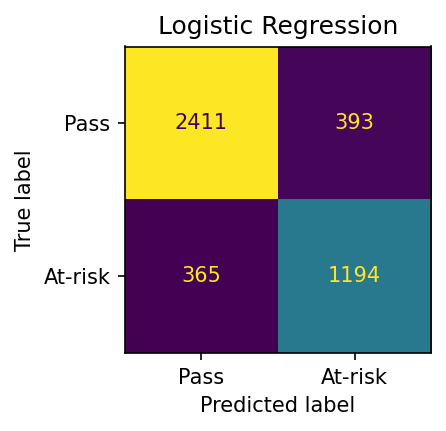
\includegraphics[width=\textwidth]{cm_logreg_full.png}
    \caption{Logistic Regression}
  \end{subfigure}
  \hfill
  \begin{subfigure}[b]{0.48\textwidth}
    \centering
    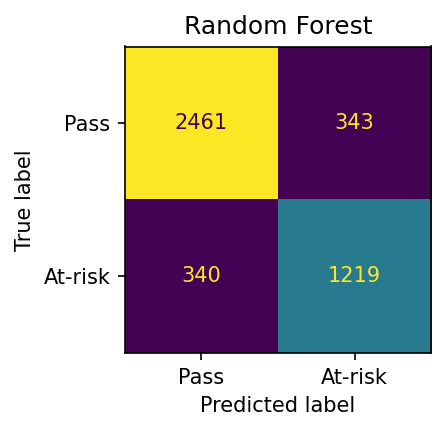
\includegraphics[width=\textwidth]{cm_rf_full.png}
    \caption{Random Forest}
  \end{subfigure}\\[0.6em]
  \begin{subfigure}[b]{0.48\textwidth}
    \centering
    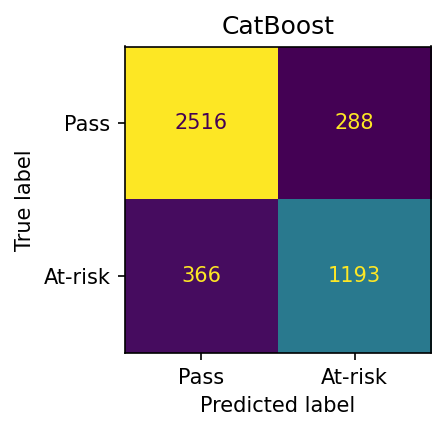
\includegraphics[width=\textwidth]{cm_catboost_full.png}
    \caption{CatBoost}
  \end{subfigure}
  \hfill
  \begin{subfigure}[b]{0.48\textwidth}
    \centering
    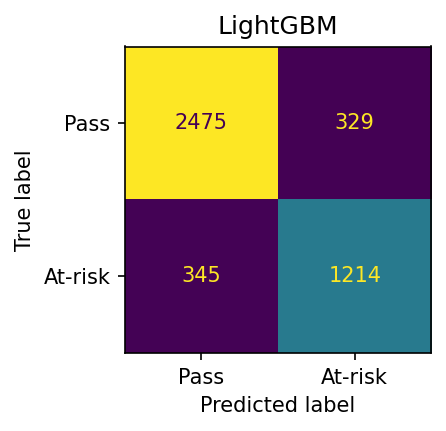
\includegraphics[width=\textwidth]{cm_lgbm_full.png}
    \caption{LightGBM}
  \end{subfigure}
  \caption{Ma trận nhầm lẫn trên tập kiểm tra --- bộ đặc trưng đầy đủ
  , tại mốc 150 ngày.}
  \label{fig:cm_full}
\end{figure}

Nhìn chung, phần lớn sai số của cả bốn mô hình đều nằm ở việc \textbf{bỏ sót
sinh viên At-risk} (dự báo Pass trong khi thực tế At-risk) nhiều hơn là cảnh
báo nhầm (dự báo At-risk trong khi thực tế Pass). Đây là điểm cần lưu ý khi
triển khai thực tế: có thể cân nhắc hạ ngưỡng phân loại để tăng recall, chấp
nhận đánh đổi thêm một số cảnh báo nhầm nhằm giảm thiểu rủi ro bỏ sót sinh
viên cần hỗ trợ.

\section{Độ quan trọng của đặc trưng}

Hình~\ref{fig:feat_imp} thể hiện độ quan trọng đặc trưng theo định nghĩa riêng
của từng thuật toán (hệ số hồi quy tuyệt đối với Logistic Regression, độ giảm
tạp chất Gini với Random Forest, PredictionValuesChange với CatBoost, và số
lần được dùng để phân tách với LightGBM) --- các giá trị này \textbf{không
cùng đơn vị} nên chỉ so sánh được thứ hạng, không so sánh trực tiếp độ lớn
giữa các mô hình.

\begin{figure}[H]
  \centering
  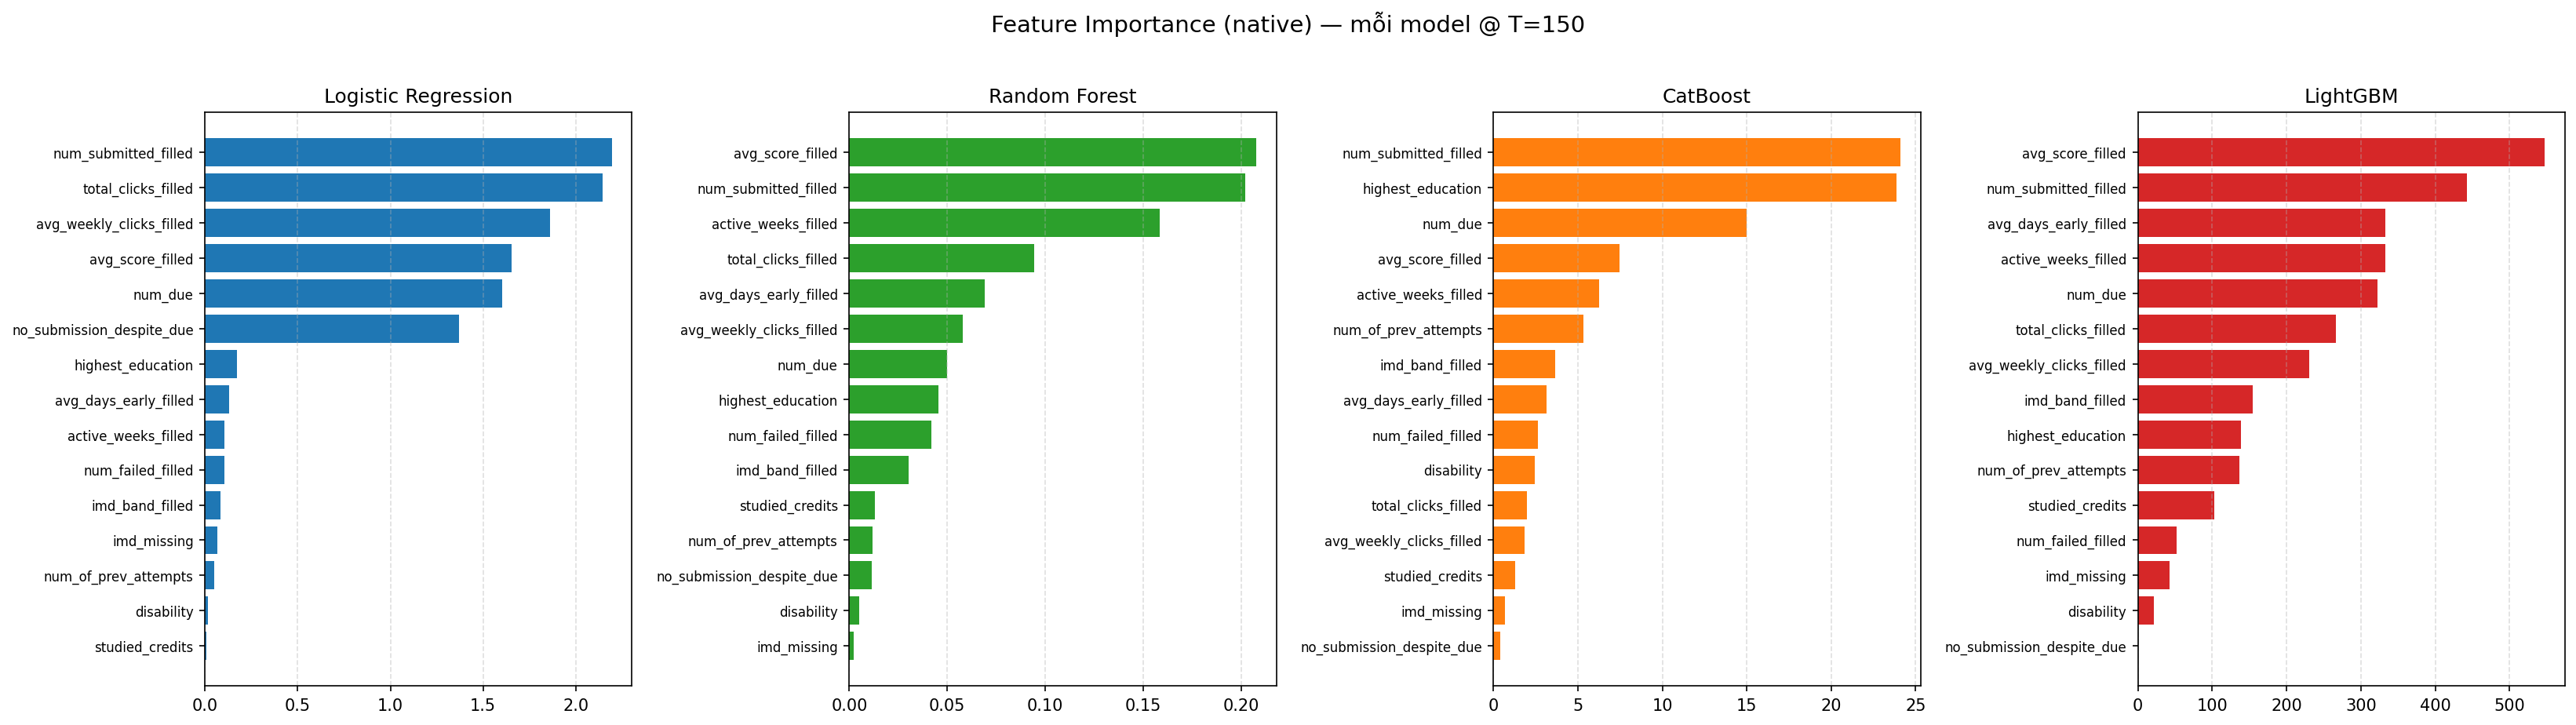
\includegraphics[width=\textwidth]{feature_importance_native.png}
  \caption{Độ quan trọng đặc trưng (theo định nghĩa riêng của từng mô hình) tại
  mốc 150 ngày.}
  \label{fig:feat_imp}
\end{figure}

Để tổng hợp một thứ hạng chung, mỗi đặc trưng được xếp hạng riêng trong từng
mô hình rồi lấy trung bình cộng bốn hạng. Bảng~\ref{tab:feature_rank} trình bày
kết quả, sắp xếp tăng dần theo hạng trung bình.

\begin{table}[H]
  \centering
  \caption{Thứ hạng độ quan trọng của từng đặc trưng theo mỗi mô hình (1 = quan trọng nhất) và hạng trung bình, sắp xếp tăng dần theo hạng trung bình.}
  \label{tab:feature_rank}
  \footnotesize
  \begin{tabular}{lrrrrr}
    \toprule
    \textbf{Đặc trưng} & \textbf{LogReg} & \textbf{RF} & \textbf{CatBoost} & \textbf{LightGBM} & \textbf{Hạng TB} \\
    \midrule
    \code{num\_submitted\_filled} & 1 & 1 & 1 & 3 & 1.50 \\
    \code{avg\_score\_filled} & 5 & 2 & 4 & 1 & 3.00 \\
    \code{num\_due} & 4 & 7 & 3 & 7 & 5.25 \\
    \code{total\_clicks\_filled} & 2 & 4 & 10 & 6 & 5.50 \\
    \code{active\_weeks\_filled} & 9 & 3 & 6 & 4 & 5.50 \\
    \code{highest\_education} & 7 & 8 & 2 & 9 & 6.50 \\
    \code{avg\_days\_early\_filled} & 11 & 6 & 8 & 2 & 6.75 \\
    \code{avg\_weekly\_clicks\_filled} & 3 & 9 & 11 & 5 & 7.00 \\
    \code{num\_failed\_filled} & 8 & 5 & 7 & 12 & 8.00 \\
    \code{imd\_band\_filled} & 10 & 11 & 9 & 8 & 9.50 \\
    \code{num\_of\_prev\_attempts} & 13 & 12 & 5 & 11 & 10.25 \\
    \code{no\_submission\_despite\_due} & 6 & 10 & 15 & 15 & 11.50 \\
    \code{studied\_credits} & 15 & 13 & 13 & 10 & 12.75 \\
    \code{disability} & 14 & 14 & 12 & 14 & 13.50 \\
    \code{imd\_missing} & 12 & 15 & 14 & 13 & 13.50 \\
    \bottomrule
  \end{tabular}
\end{table}


\begin{itemize}[leftmargin=*]
  \item \textbf{Nhóm dẫn đầu} --- \code{num\_submitted\_filled} (số bài đã
        nộp) đứng hạng 1 ở Logistic Regression và CatBoost, hạng 2 ở Random
        Forest và LightGBM (hạng trung bình 1.50), khẳng định đây là tín hiệu
        dự báo mạnh và nhất quán nhất. Theo sau là \code{avg\_score\_filled}
        (điểm trung bình, hạng trung bình 2.50 --- dẫn đầu ở Random Forest và
        LightGBM), rồi đến \code{num\_due} (số bài đến hạn) và
        \code{active\_weeks\_filled} (số tuần hoạt động) cùng ở hạng trung
        bình 5.00. Cả bốn đều là đặc trưng \textbf{động}, phản ánh trực tiếp
        mức độ tham gia và kết quả học tập tích luỹ.
  \item \textbf{Nhóm giữa} gồm các đặc trưng tương tác VLE còn lại
        (\code{total\_clicks\_filled}, \code{avg\_weekly\_clicks\_filled}),
        \code{avg\_days\_early\_filled} và \code{highest\_education} --- đóng
        góp bổ sung nhưng không mang tính quyết định.
  \item \textbf{Nhóm cuối} --- \code{studied\_credits}, \code{disability},
        \code{imd\_missing} có hạng trung bình cao nhất (ít quan trọng nhất),
        cho thấy các đặc trưng tĩnh mang tính nhân khẩu học có vai trò dự báo
        khiêm tốn hơn nhiều so với các đặc trưng hành vi động.
\end{itemize}

\section{Rút gọn đặc trưng: Top-10 và Top-5}

Dựa trên thứ hạng ở Bảng~\ref{tab:feature_rank}, mười đặc trưng quan trọng
nhất (Top-10) và năm đặc trưng quan trọng nhất (Top-5) được chọn ra để huấn
luyện lại theo đúng quy trình tinh chỉnh đã mô tả ở Mục~3, nhằm kiểm tra hiệu
suất mô hình có \textbf{ổn định} hay không khi giảm số lượng đặc trưng đầu
vào --- một yếu tố quan trọng khi triển khai hệ thống cảnh báo thực tế, nơi
việc thu thập và duy trì ít đặc trưng hơn giúp đơn giản hoá quy trình vận hành.

Bảng~\ref{tab:compare_top10} và Bảng~\ref{tab:compare_top5} trình bày kết quả
tương ứng với hai bộ đặc trưng rút gọn.

\begin{table}[H]
  \centering
  \caption{So sánh các mô hình sau khi rút gọn về 10 đặc trưng quan trọng nhất (Top-10).}
  \label{tab:compare_top10}
  \small
  \setlength{\tabcolsep}{5pt}
  \begin{tabular}{lrrrrr}
    \toprule
    \textbf{Model} & \textbf{Accuracy} & \textbf{Precision} & \textbf{Recall} & \textbf{F1} & \textbf{ROC-AUC} \\
    \midrule
    \textbf{Logistic Regression} & 0.8260 & 0.7475 & 0.7749 & 0.7609 & 0.8966 \\
    \textbf{Random Forest} & 0.8492 & \textbf{0.8135} & 0.7498 & 0.7804 & 0.9074 \\
    \textbf{CatBoost} & \textbf{0.8501} & 0.7979 & 0.7774 & \textbf{0.7875} & \textbf{0.9119} \\
    \textbf{LightGBM} & 0.8398 & 0.7718 & \textbf{0.7832} & 0.7775 & 0.9095 \\
    \bottomrule
  \end{tabular}
\end{table}

\begin{table}[H]
  \centering
  \caption{So sánh các mô hình sau khi rút gọn về 5 đặc trưng quan trọng nhất (Top-5).}
  \label{tab:compare_top5}
  \small
  \setlength{\tabcolsep}{5pt}
  \begin{tabular}{lrrrrr}
    \toprule
    \textbf{Model} & \textbf{Accuracy} & \textbf{Precision} & \textbf{Recall} & \textbf{F1} & \textbf{ROC-AUC} \\
    \midrule
    \textbf{Logistic Regression} & 0.8529 & 0.7876 & 0.7675 & 0.7775 & 0.9148 \\
    \textbf{Random Forest} & \textbf{0.8700} & \textbf{0.8116} & 0.7966 & \textbf{0.8040} & 0.9279 \\
    \textbf{CatBoost} & 0.8667 & 0.7979 & \textbf{0.8058} & 0.8018 & \textbf{0.9302} \\
    \textbf{LightGBM} & 0.8626 & 0.7950 & 0.7945 & 0.7948 & 0.9286 \\
    \bottomrule
  \end{tabular}
\end{table}


Hình~\ref{fig:cm_grid} tổng hợp ma trận nhầm lẫn của toàn bộ 8 tổ hợp (bộ đặc
trưng $\times$ mô hình) trên cùng một lưới để tiện đối chiếu.

\begin{figure}[H]
  \centering
  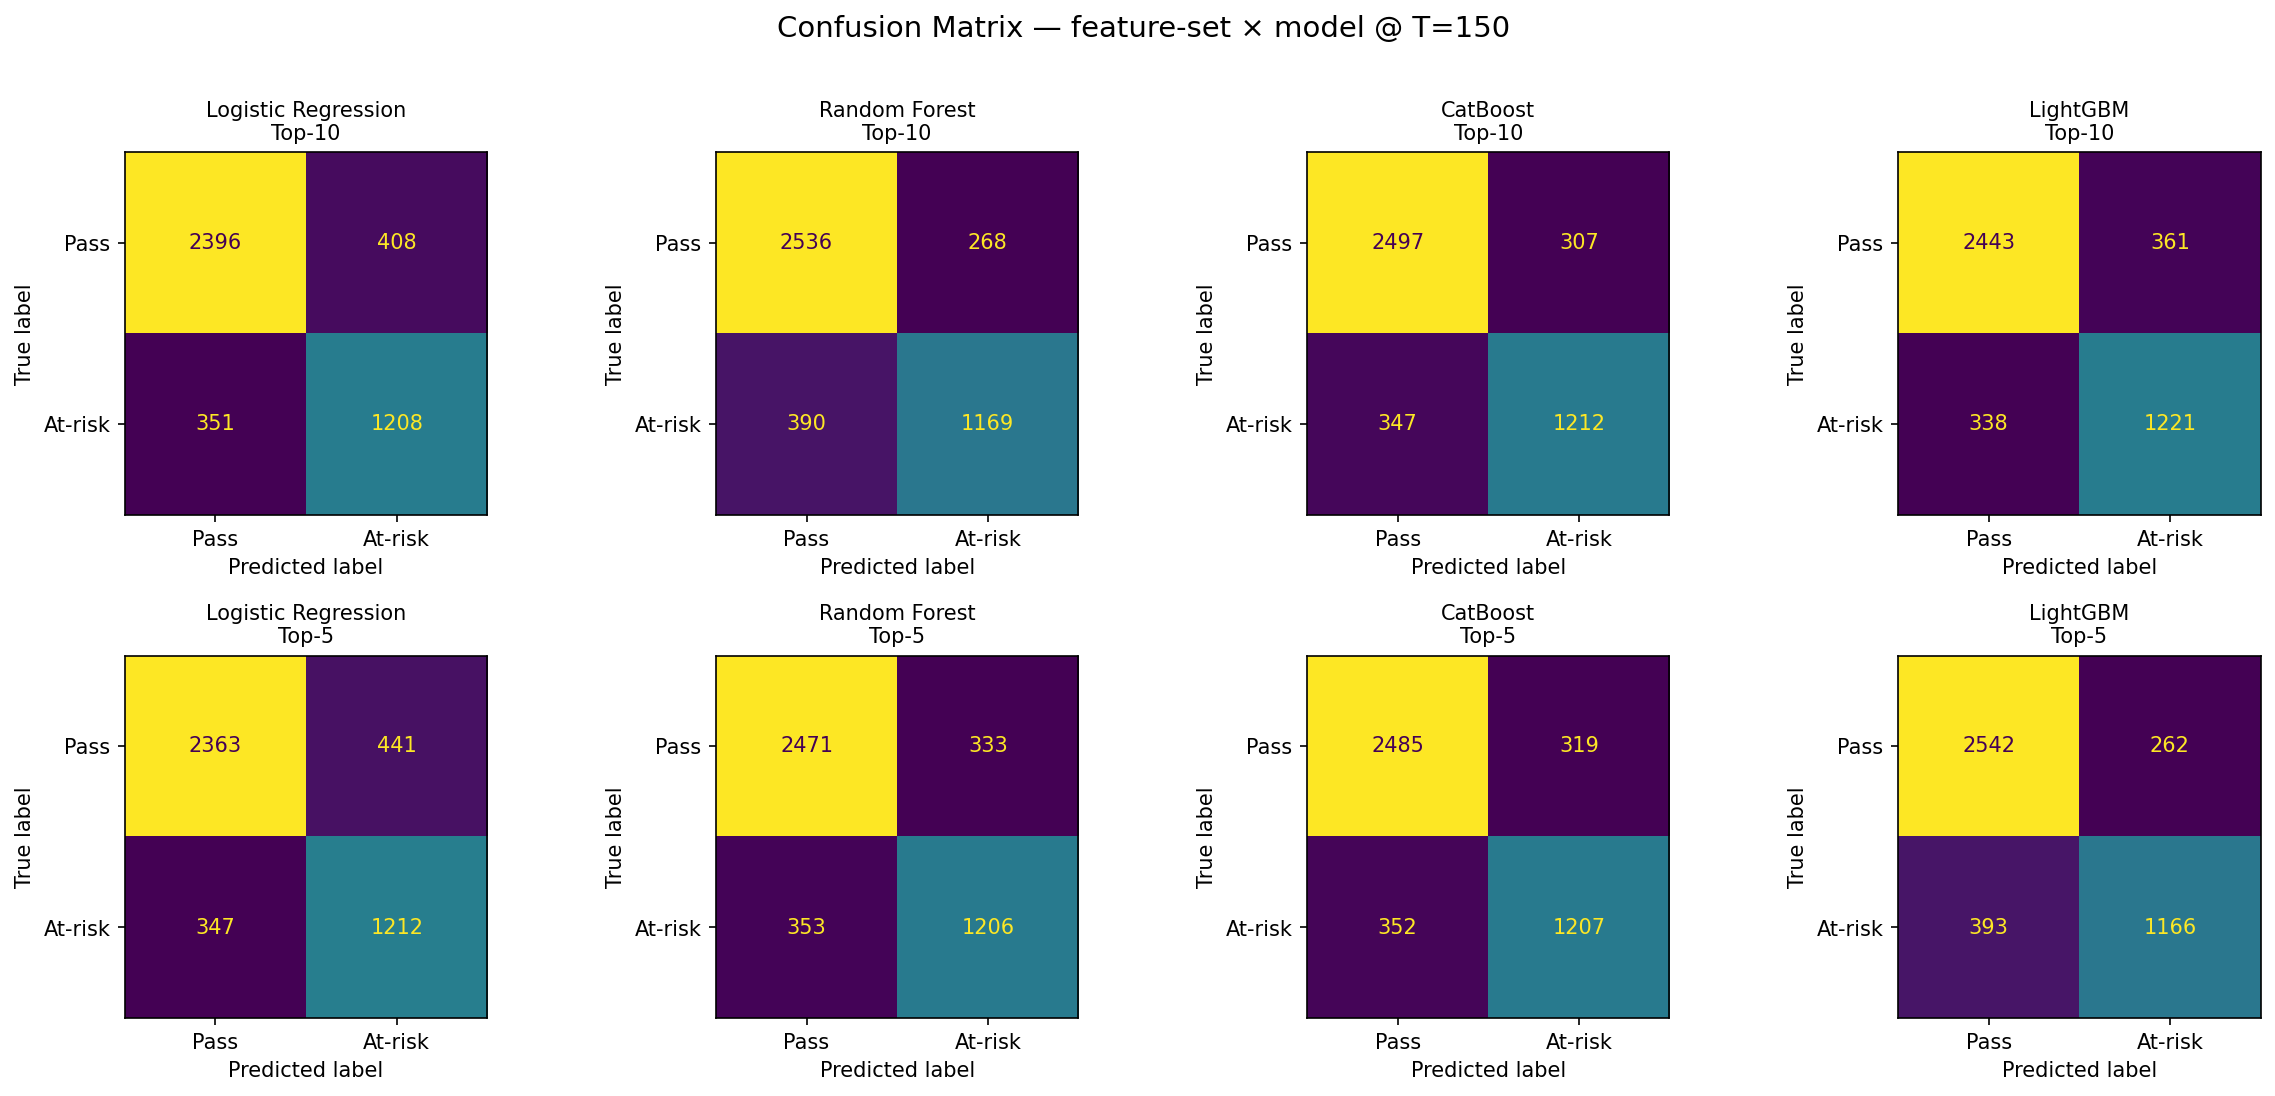
\includegraphics[width=\textwidth]{cm_grid_topn.png}
  \caption{Ma trận nhầm lẫn của bốn mô hình trên hai bộ đặc trưng rút gọn
  Top-10 và Top-5, tại mốc 150 ngày.}
  \label{fig:cm_grid}
\end{figure}

Hình~\ref{fig:stability} theo dõi sự biến động của cả năm chỉ số khi số lượng
đặc trưng giảm dần từ 15 xuống 10 rồi 5.

\begin{figure}[H]
  \centering
  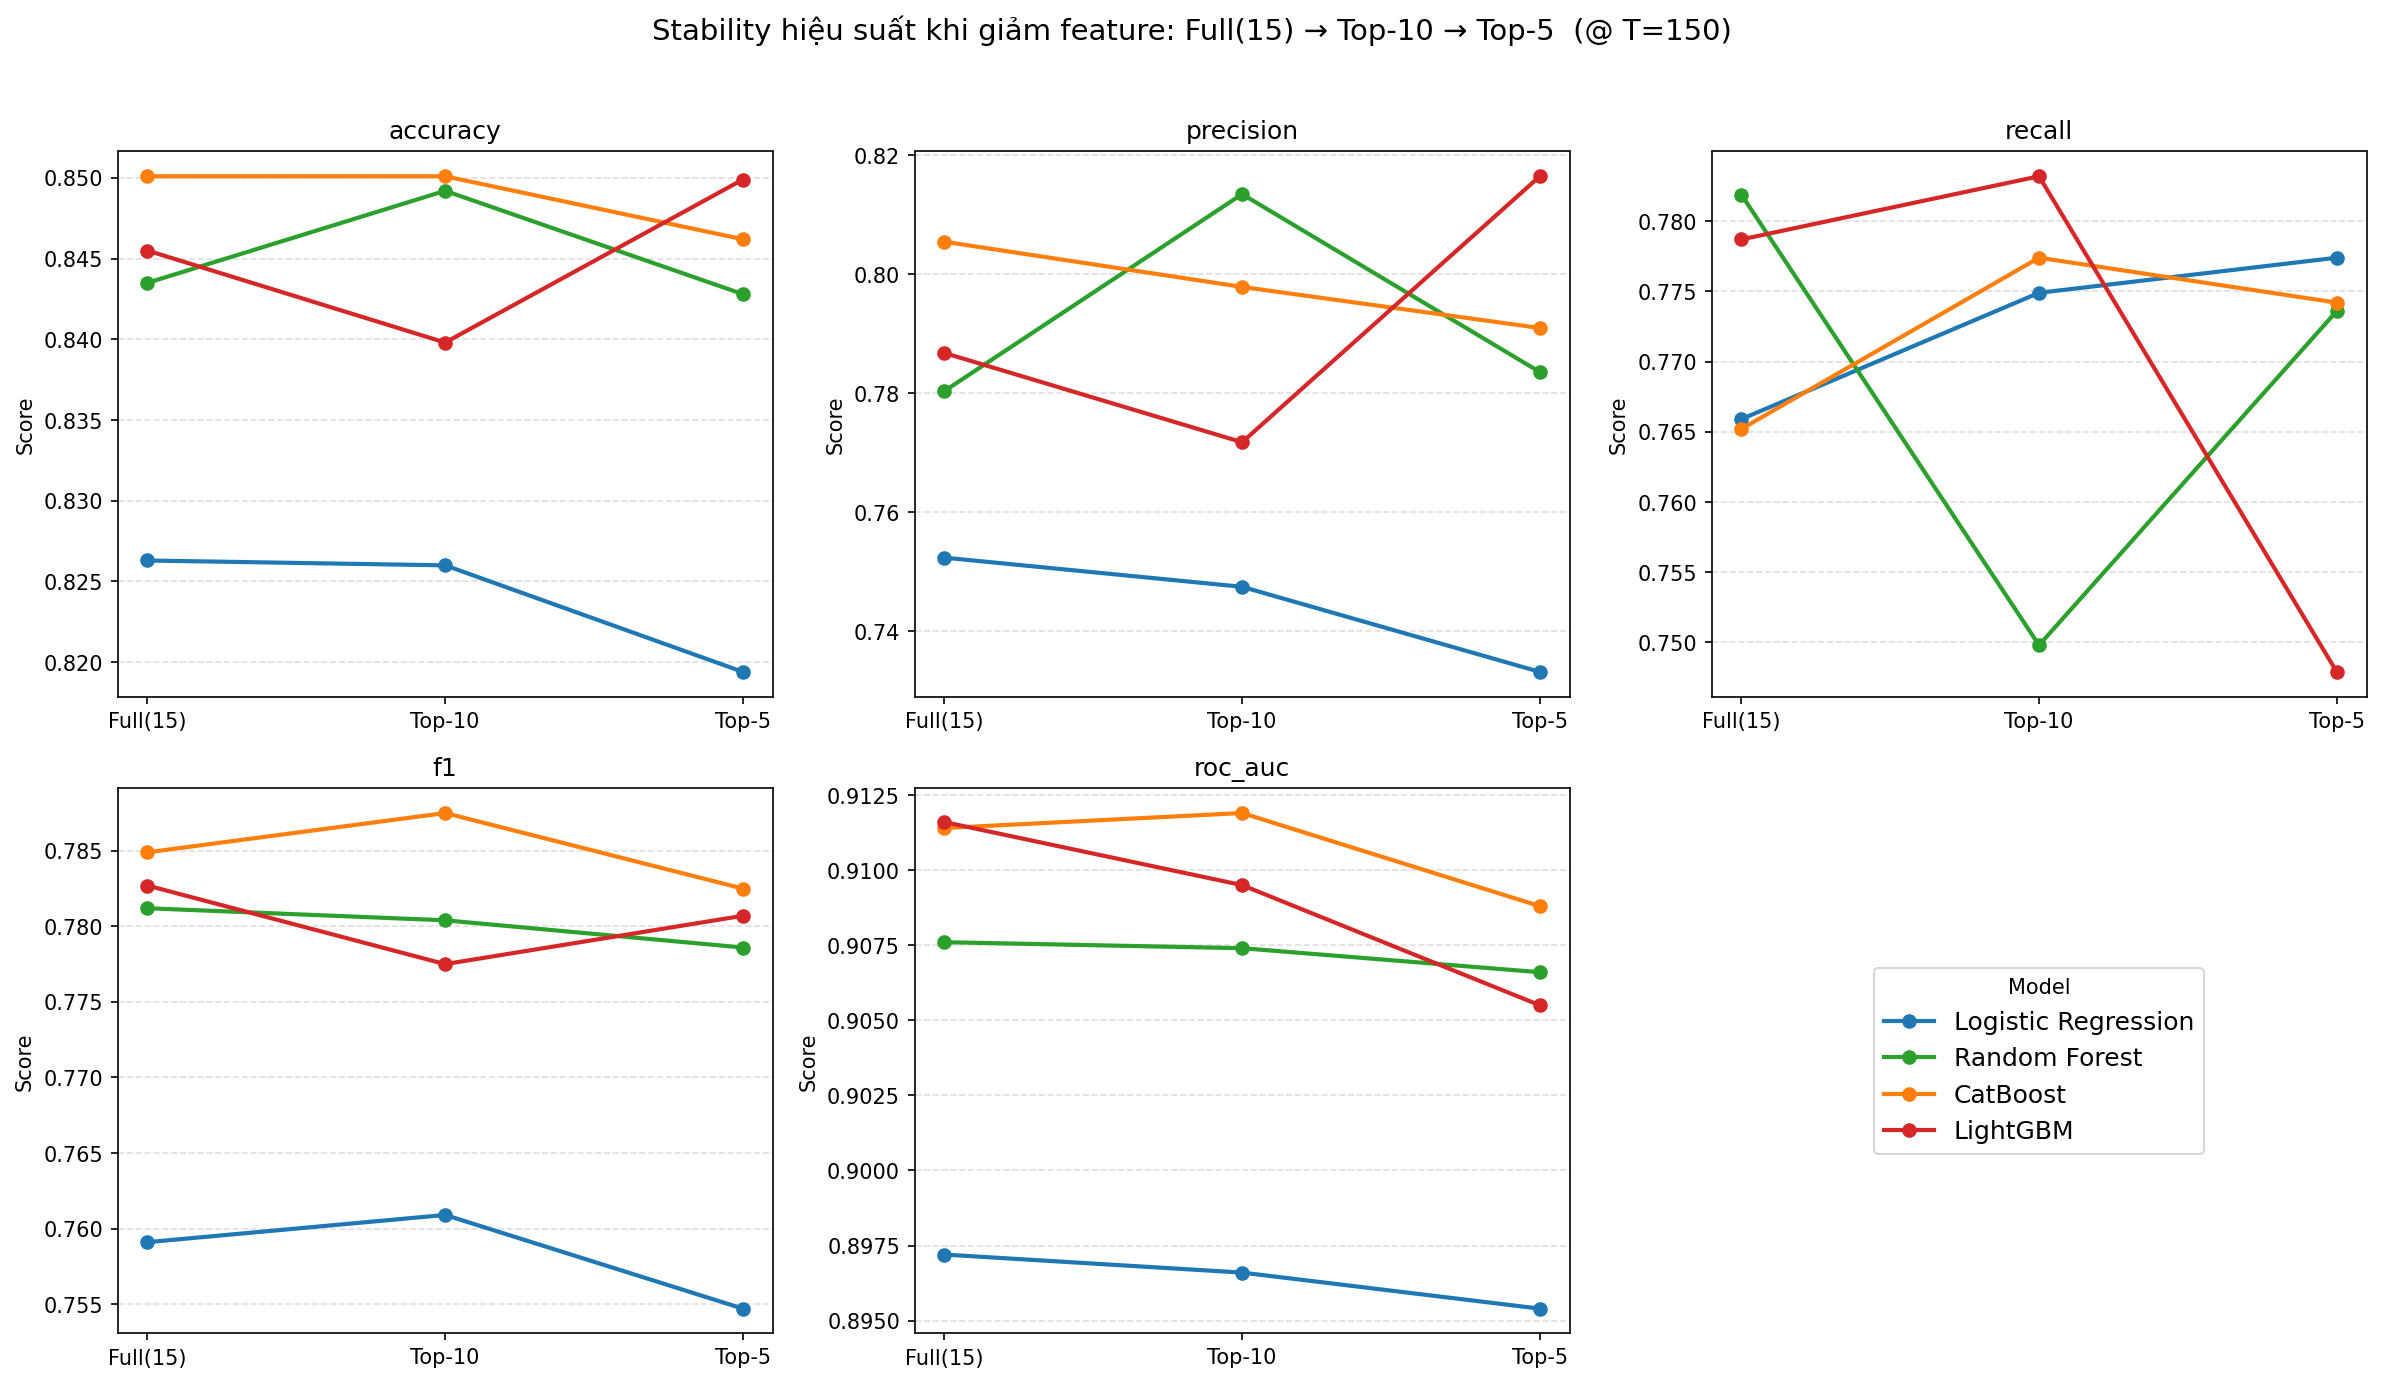
\includegraphics[width=0.95\textwidth]{stability_featureset.png}
  \caption{Biến động các chỉ số hiệu suất khi giảm số lượng đặc trưng:
  Full(15) $\to$ Top-10 $\to$ Top-5, tại mốc 150 ngày.}
  \label{fig:stability}
\end{figure}

\begin{itemize}[leftmargin=*]
  \item Hiệu suất của cả bốn mô hình \textbf{rất ổn định} qua ba bộ đặc trưng
        --- không có chỉ số nào sụt giảm đáng kể khi giảm từ 15 xuống chỉ còn
        5 đặc trưng. Điều này khẳng định thêm kết luận ở Mục~5: phần lớn sức
        mạnh dự báo tập trung ở một nhóm nhỏ đặc trưng hành vi động.
  \item Đáng chú ý, \textbf{CatBoost ở bộ Top-10 đạt F1 At-risk cao nhất trong
        toàn bộ thực nghiệm} (0.7875), nhỉnh hơn chính nó ở bộ đặc trưng đầy
        đủ (0.7849). Mô hình này cũng cải thiện recall khi giảm đặc trưng (từ
        0.7652 ở Full lên 0.7774 ở Top-10) --- tức việc loại bỏ các đặc trưng
        nhiễu giúp bắt được nhiều sinh viên có nguy cơ hơn.
  \item \textbf{Logistic Regression} là mô hình duy nhất suy giảm rõ ở
        accuracy và precision khi cắt bớt đặc trưng (accuracy 0.8263 $\to$
        0.8194; precision 0.7524 $\to$ 0.7332 khi đi từ Full xuống Top-5) ---
        phù hợp với đặc tính tuyến tính: mô hình này hưởng lợi từ việc có
        nhiều biến hơn để bù đắp cho khả năng nắm bắt tương tác hạn chế.
\end{itemize}

Hình~\ref{fig:f1_bar} so sánh trực tiếp F1 At-risk giữa Top-10 và Top-5 cho
từng mô hình.

\begin{figure}[H]
  \centering
  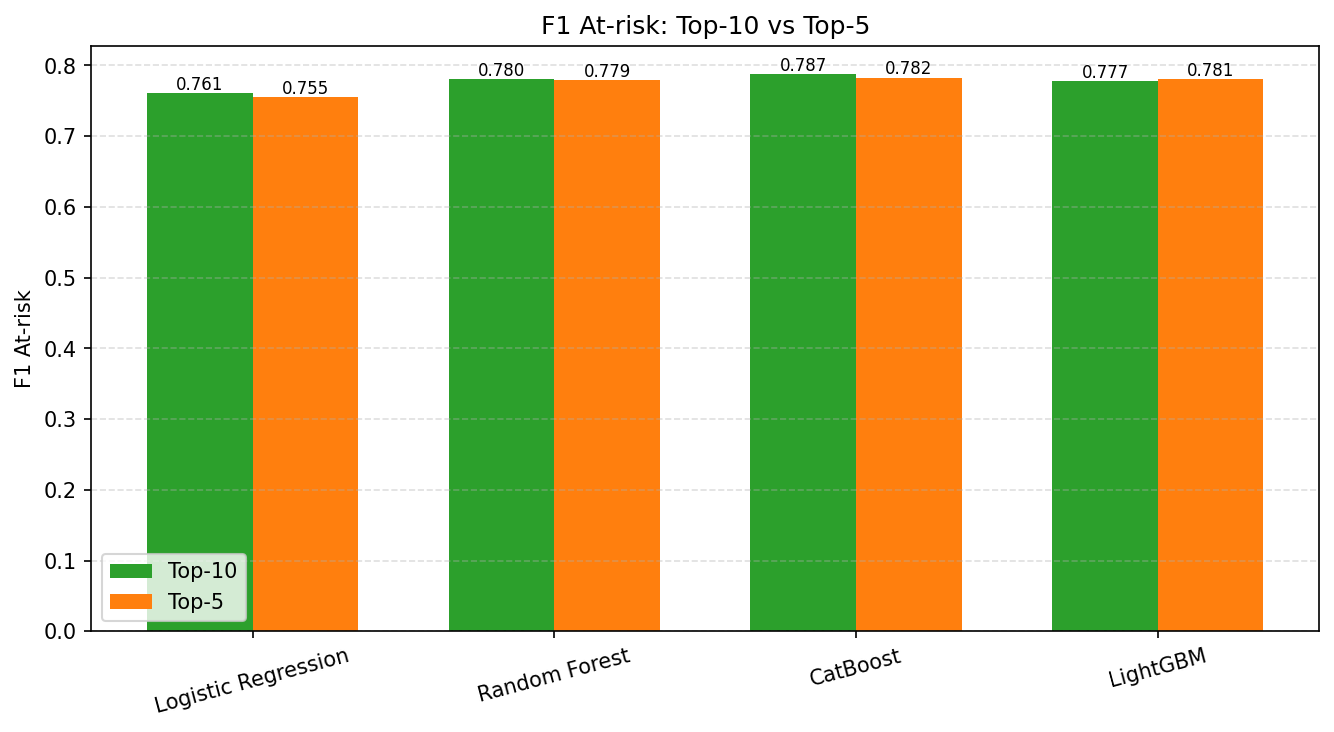
\includegraphics[width=0.8\textwidth]{f1_top10_vs_top5.png}
  \caption{So sánh F1 At-risk giữa bộ Top-10 và Top-5 theo từng mô hình.}
  \label{fig:f1_bar}
\end{figure}

Chênh lệch F1 giữa hai bộ đặc trưng rút gọn đều nhỏ hơn 0.01 ở mọi mô hình,
củng cố nhận định rằng \textbf{bộ Top-5 là lựa chọn hợp lý cho triển khai thực
tế}, cân bằng tốt giữa hiệu suất và chi phí thu thập/duy trì đặc trưng.

Cuối cùng, Bảng~\ref{tab:best_params} tổng hợp siêu tham số liên quan đến xử lý
mất cân bằng nhãn mà Optuna lựa chọn cho từng mô hình, ở cả ba bộ đặc trưng.

\begin{table}[H]
  \centering
  \caption{Siêu tham số tối ưu liên quan đến xử lý mất cân bằng nhãn --- tỷ lệ oversampling SMOTE và trọng số lớp At-risk --- được Optuna lựa chọn cho từng mô hình và từng bộ đặc trưng, cùng F1 At-risk trung bình qua 3-fold cross-validation.}
  \label{tab:best_params}
  \small
  \resizebox{\textwidth}{!}{%
  \begin{tabular}{llrrr}
    \toprule
    \textbf{Bộ đặc trưng} & \textbf{Model} & \textbf{F1 At-risk (CV)} & \textbf{Tỷ lệ SMOTE} & \textbf{Trọng số At-risk} \\
    \midrule
    \multirow{4}{*}{Full (15)} & \textbf{Logistic Regression} & 0.7767 & +0.55x & 1.05 \\
     & \textbf{Random Forest} & 0.7836 & +0.56x & 1.70 \\
     & \textbf{CatBoost} & 0.7899 & +0.63x & 1.27 \\
     & \textbf{LightGBM} & 0.7894 & +0.17x & 1.55 \\
    \midrule
    \multirow{4}{*}{Top-10} & \textbf{Logistic Regression} & 0.7768 & +0.62x & 1.11 \\
     & \textbf{Random Forest} & 0.7819 & +0.48x & 1.04 \\
     & \textbf{CatBoost} & 0.7903 & +0.57x & 1.33 \\
     & \textbf{LightGBM} & 0.7887 & +0.21x & 1.63 \\
    \midrule
    \multirow{4}{*}{Top-5} & \textbf{Logistic Regression} & 0.7741 & +0.67x & 1.12 \\
     & \textbf{Random Forest} & 0.7882 & +0.50x & 1.27 \\
     & \textbf{CatBoost} & 0.7894 & +0.57x & 1.33 \\
     & \textbf{LightGBM} & 0.7867 & +0.34x & 1.11 \\
    \bottomrule
  \end{tabular}}
\end{table}


Xu hướng chung: các mô hình cây (Random Forest, CatBoost, LightGBM) có trọng
số At-risk tối ưu dao động rộng (1.04--1.70) tuỳ mô hình và bộ đặc trưng, trong
khi Logistic Regression luôn hội tụ về trọng số gần 1.0 (1.05--1.12) và tỷ lệ
SMOTE tương đối cao (0.55--0.67x) --- mô hình tuyến tính dựa nhiều hơn vào việc
tạo thêm mẫu tổng hợp thay vì điều chỉnh trọng số lớp để xử lý mất cân bằng. Ở
chiều ngược lại, LightGBM là mô hình cần ít mẫu tổng hợp nhất (tỷ lệ SMOTE chỉ
0.17--0.34x) nhưng lại dùng trọng số lớp cao hơn, cho thấy mỗi thuật toán có
cách riêng để bù đắp cho sự mất cân bằng nhãn.

\section{Diễn giải mô hình bằng SHAP}

Để hiểu sâu hơn cơ chế ra quyết định của mô hình, phương pháp \textbf{SHAP}
(SHapley Additive exPlanations) được áp dụng cho mô hình có F1 At-risk cao
nhất trên bộ đặc trưng đầy đủ --- \textbf{CatBoost} --- trên cả ba bộ đặc
trưng (Full, Top-10, Top-5) để đối chiếu mức độ nhất quán của các diễn giải
khi số lượng đặc trưng thay đổi.

\subsection{Biểu đồ tổng quan (beeswarm và mean\texorpdfstring{$|$}{|}SHAP\texorpdfstring{$|$}{|})}

Hình~\ref{fig:shap_full} trình bày kết quả SHAP trên bộ đặc trưng đầy đủ: biểu
đồ beeswarm cho biết chiều và độ phân tán ảnh hưởng của từng đặc trưng lên
từng sinh viên cụ thể, trong khi biểu đồ cột thể hiện mức độ quan trọng trung
bình.

\begin{figure}[H]
  \centering
  \begin{subfigure}[b]{0.58\textwidth}
    \centering
    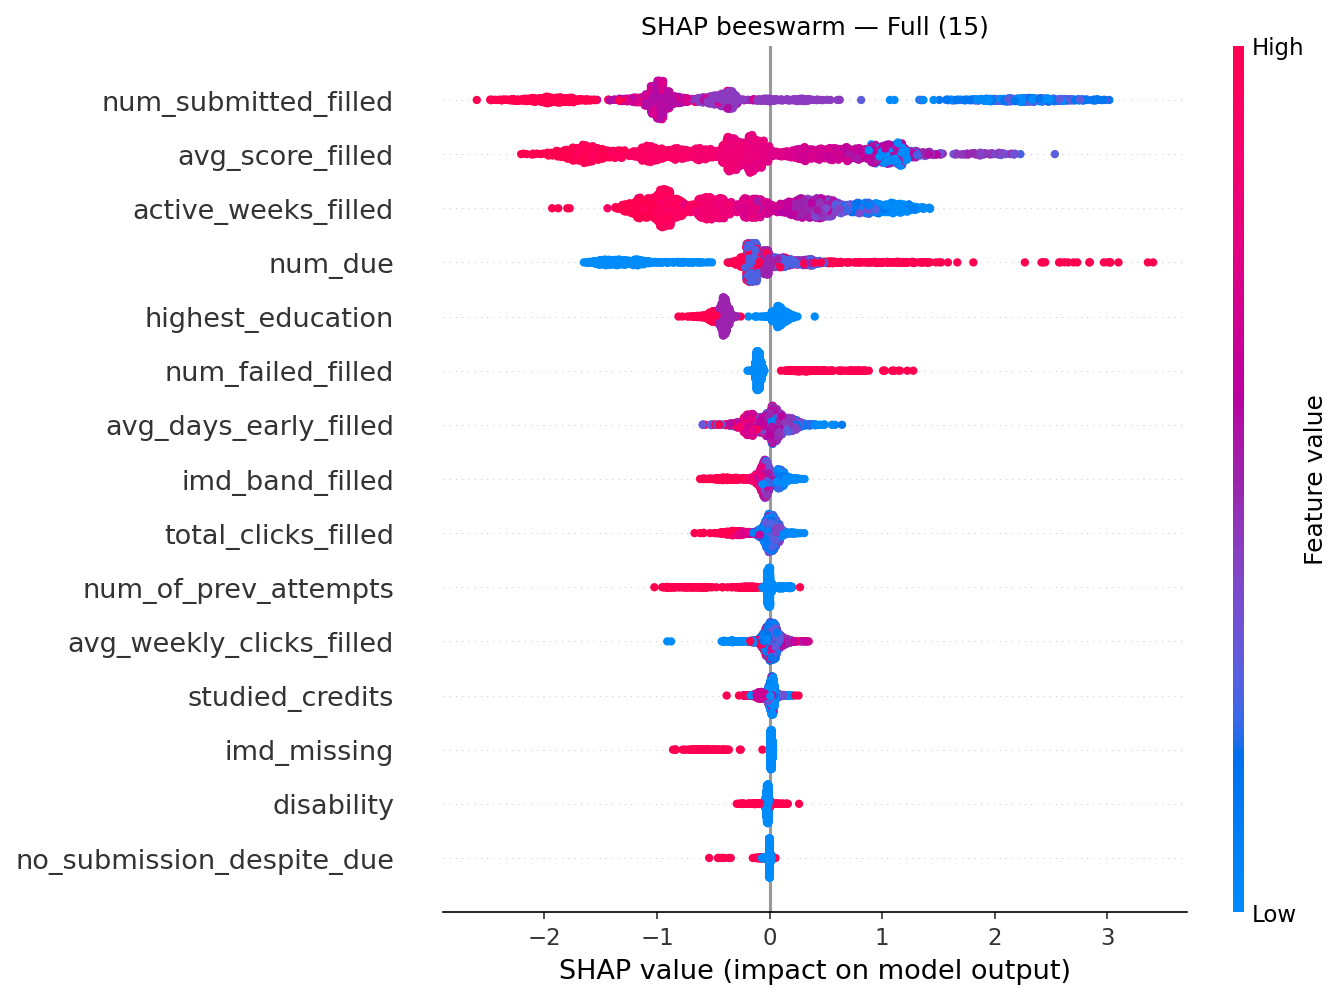
\includegraphics[width=\textwidth]{shap_beeswarm_full.png}
    \caption{Beeswarm}
  \end{subfigure}
  \hfill
  \begin{subfigure}[b]{0.38\textwidth}
    \centering
    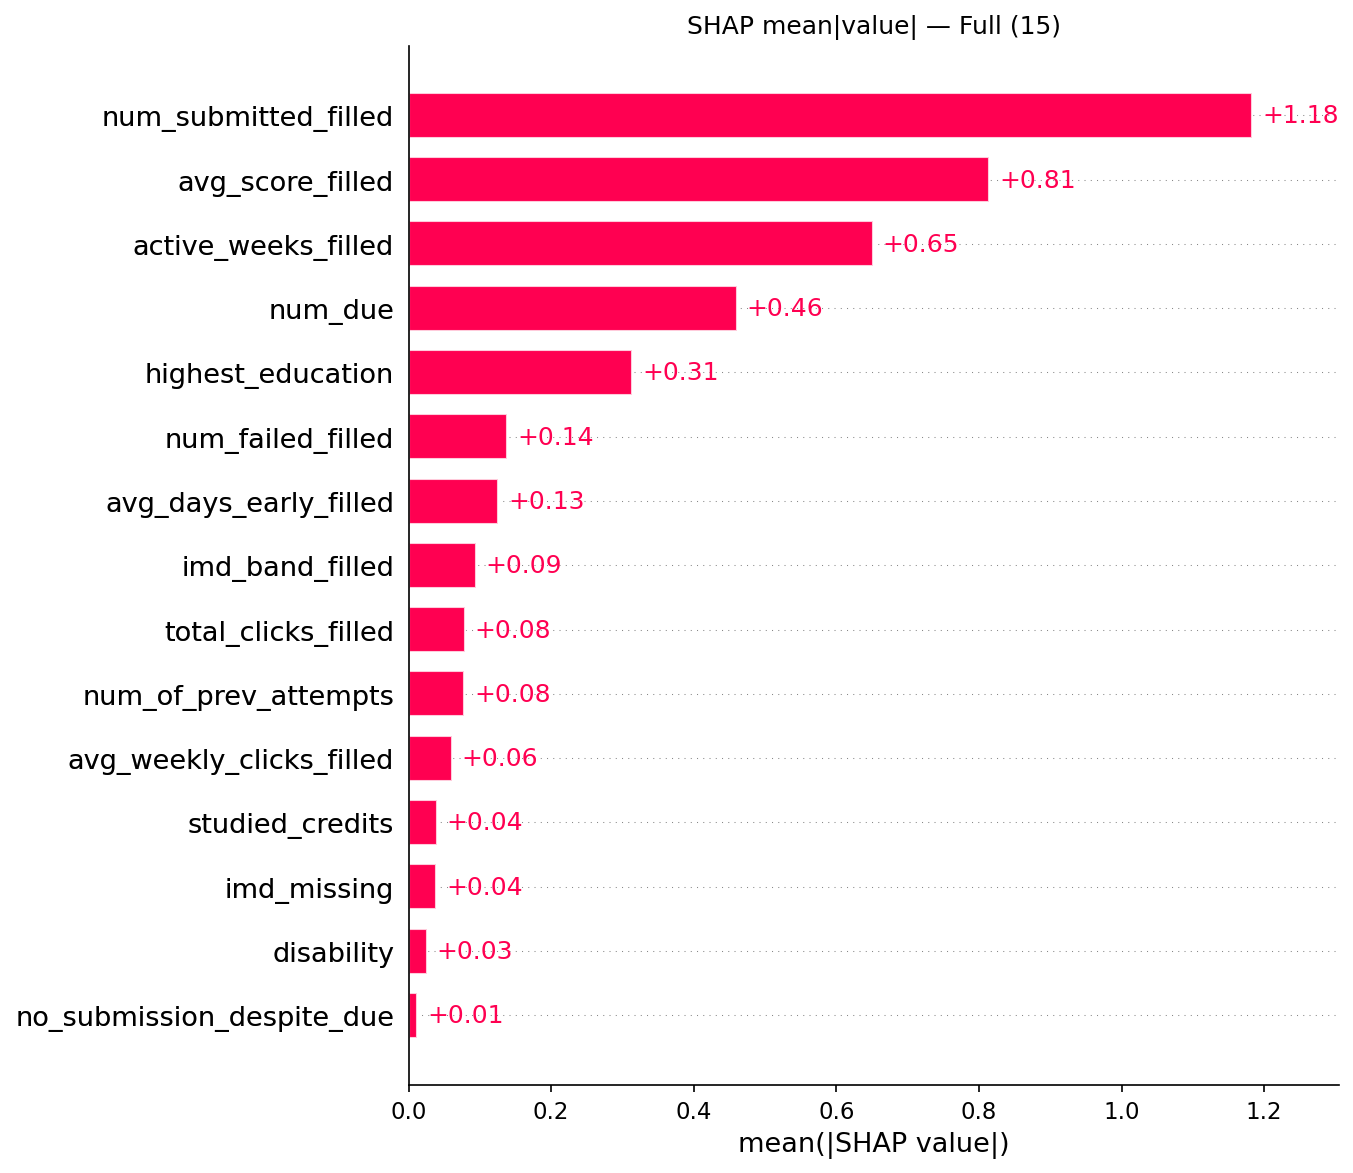
\includegraphics[width=\textwidth]{shap_bar_full.png}
    \caption{Mean $|$SHAP$|$}
  \end{subfigure}
  \caption{Diễn giải SHAP của CatBoost trên bộ đặc trưng đầy đủ (15 đặc
  trưng).}
  \label{fig:shap_full}
\end{figure}

Kết quả SHAP đồng thuận cao với thứ hạng độ quan trọng đặc trưng gốc ở
Bảng~\ref{tab:feature_rank}: \code{num\_submitted\_filled},
\code{avg\_score\_filled} và \code{active\_weeks\_filled} là ba đặc trưng có
ảnh hưởng lớn nhất. Chiều tác động phù hợp với trực giác nghiệp vụ: giá trị
\code{num\_submitted\_filled} và \code{avg\_score\_filled} \textbf{thấp}
(màu xanh) đẩy dự báo về phía \textbf{At-risk} (SHAP dương), trong khi giá trị
\textbf{cao} (màu đỏ/tím) kéo dự báo về phía Pass. Riêng \code{num\_due} (số
bài đến hạn) thể hiện chiều \textbf{ngược lại}: giá trị cao (màu đỏ) lại đẩy
về phía At-risk --- hợp lý vì số bài đến hạn cao đồng nghĩa với khối lượng
công việc dồn lại lớn, thường đi kèm nguy cơ trễ hạn hoặc bỏ bài cao hơn.

Hình~\ref{fig:shap_top10} và Hình~\ref{fig:shap_top5} lặp lại phân tích trên
với hai bộ đặc trưng rút gọn.

\begin{figure}[H]
  \centering
  \begin{subfigure}[b]{0.58\textwidth}
    \centering
    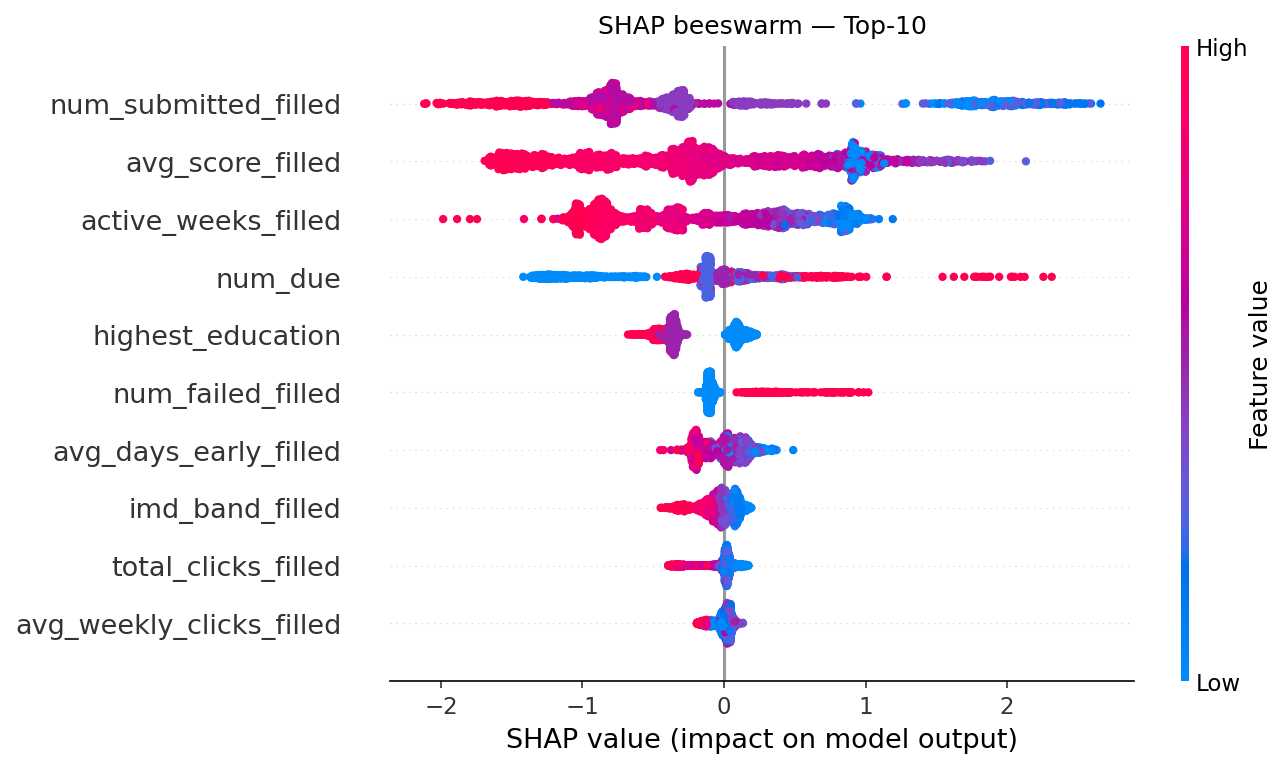
\includegraphics[width=\textwidth]{shap_beeswarm_top10.png}
    \caption{Beeswarm}
  \end{subfigure}
  \hfill
  \begin{subfigure}[b]{0.38\textwidth}
    \centering
    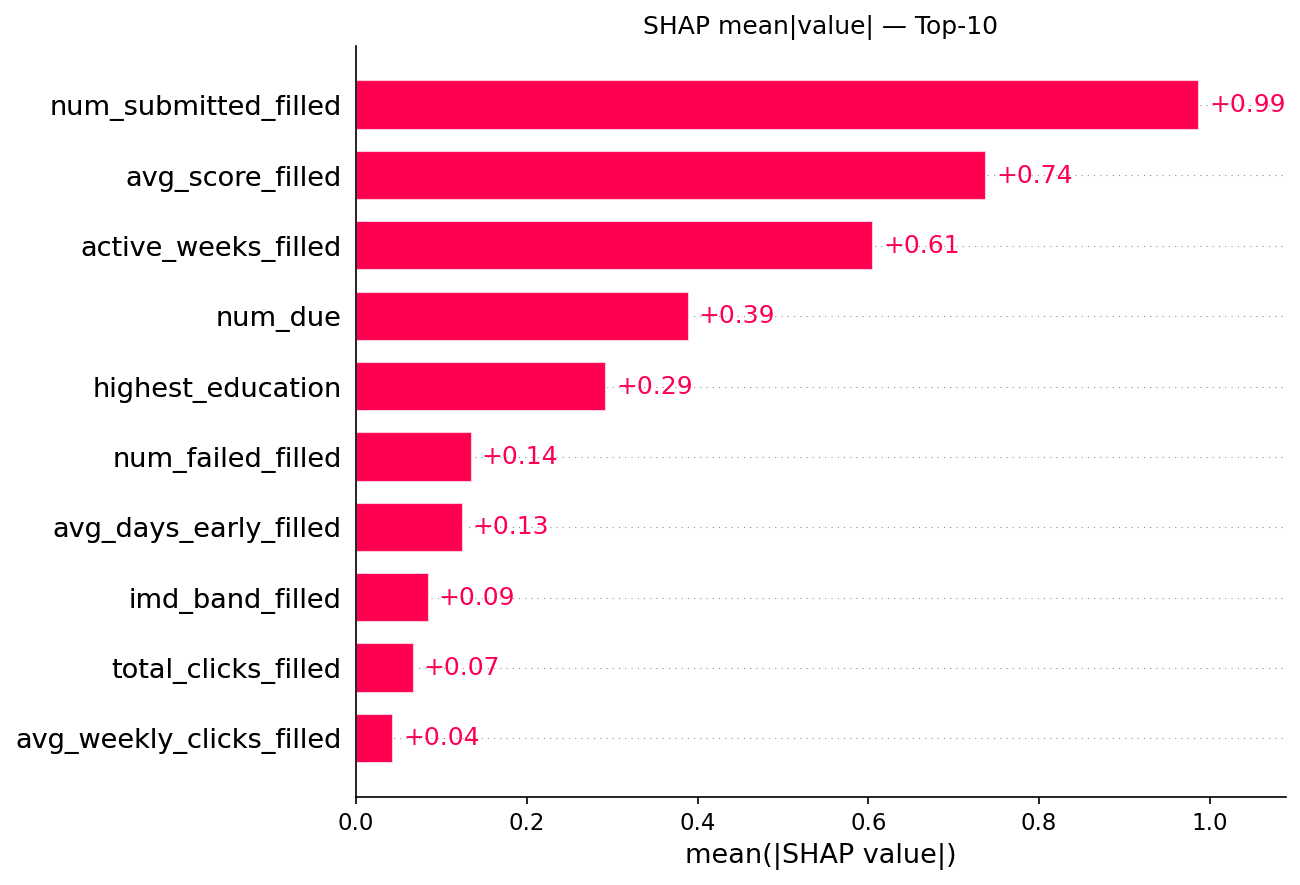
\includegraphics[width=\textwidth]{shap_bar_top10.png}
    \caption{Mean $|$SHAP$|$}
  \end{subfigure}
  \caption{Diễn giải SHAP của CatBoost trên bộ đặc trưng Top-10.}
  \label{fig:shap_top10}
\end{figure}

\begin{figure}[H]
  \centering
  \begin{subfigure}[b]{0.58\textwidth}
    \centering
    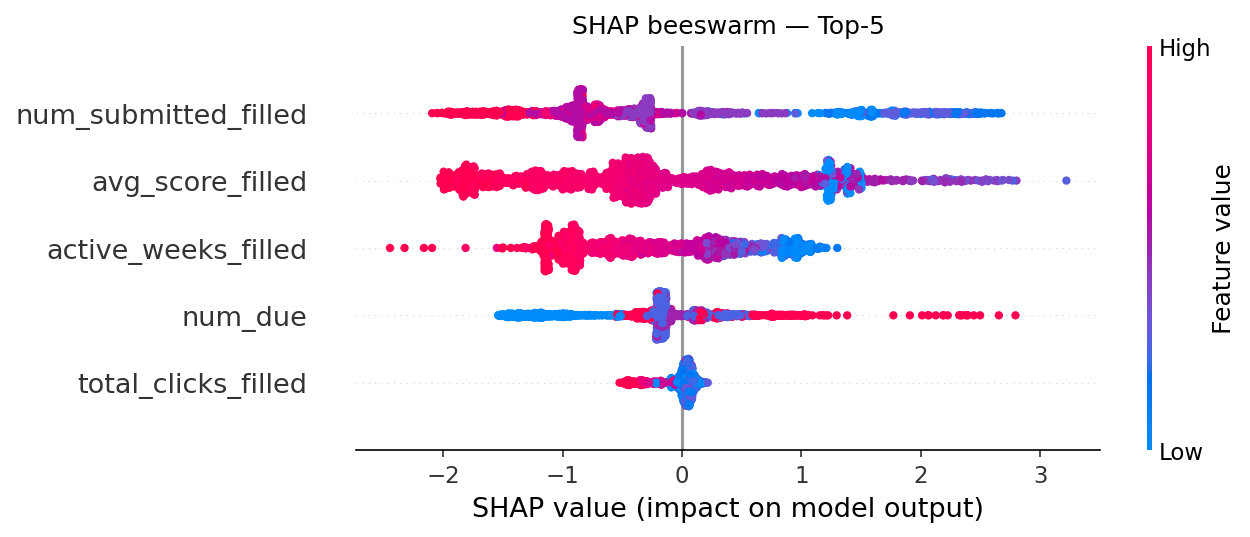
\includegraphics[width=\textwidth]{shap_beeswarm_top5.png}
    \caption{Beeswarm}
  \end{subfigure}
  \hfill
  \begin{subfigure}[b]{0.38\textwidth}
    \centering
    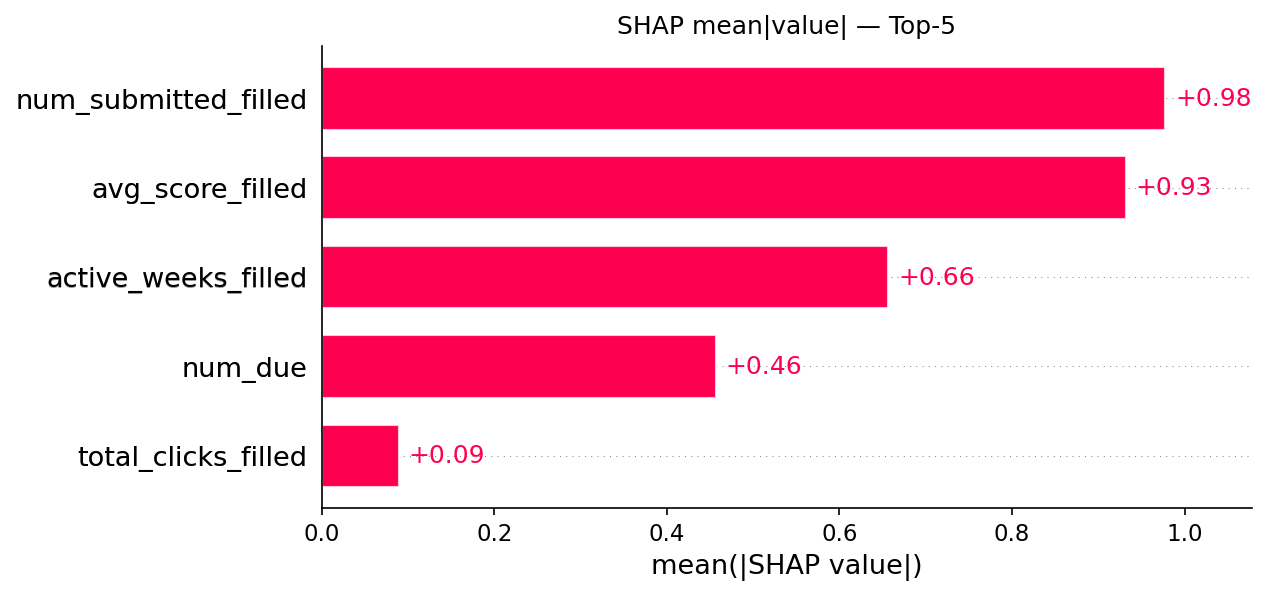
\includegraphics[width=\textwidth]{shap_bar_top5.png}
    \caption{Mean $|$SHAP$|$}
  \end{subfigure}
  \caption{Diễn giải SHAP của CatBoost trên bộ đặc trưng Top-5.}
  \label{fig:shap_top5}
\end{figure}

Thứ tự và chiều ảnh hưởng của các đặc trưng còn lại hầu như \textbf{không đổi}
khi loại bỏ dần các đặc trưng ít quan trọng --- một bằng chứng bổ sung cho
tính ổn định của mô hình đã quan sát ở Hình~\ref{fig:stability}, đồng thời cho
thấy các đặc trưng bị loại bỏ đóng góp thông tin trùng lặp hoặc không đáng kể.

\subsection{Diễn giải cục bộ: hai trường hợp minh hoạ}

Để minh hoạ cách mô hình đưa ra quyết định ở cấp độ từng cá nhân, Hình~
\ref{fig:waterfall} trình bày biểu đồ waterfall của hai sinh viên đại diện,
sử dụng mô hình CatBoost trên bộ đặc trưng đầy đủ: một trường hợp bị đẩy mạnh
về phía At-risk và một trường hợp bị đẩy mạnh về phía Pass.

\begin{figure}[H]
  \centering
  \begin{subfigure}[b]{0.48\textwidth}
    \centering
    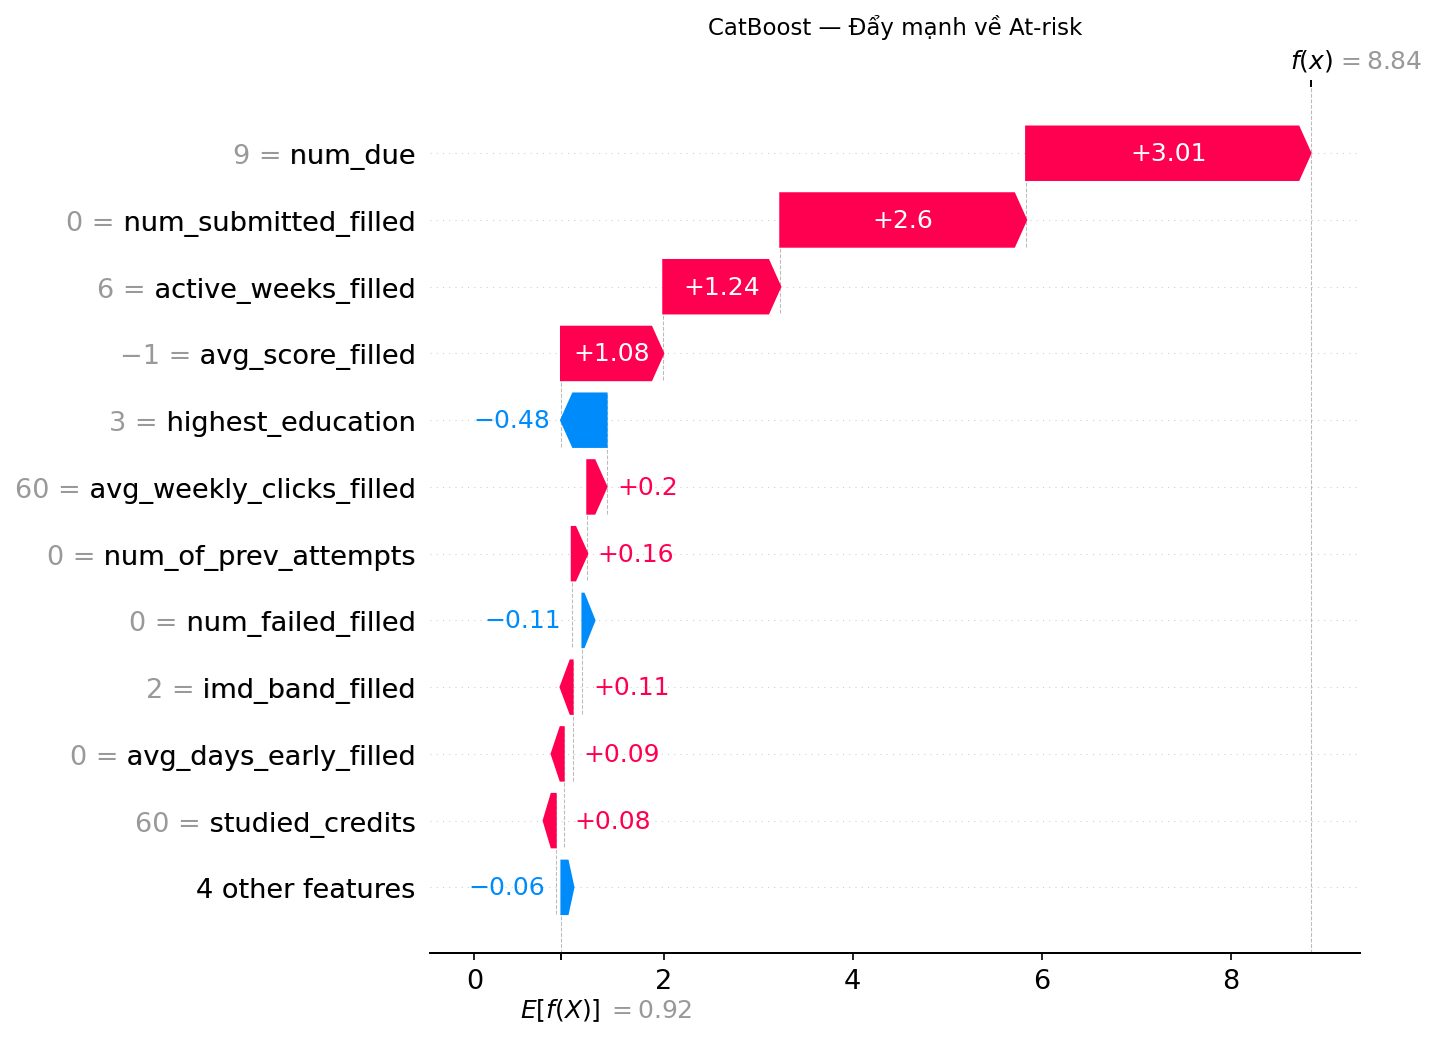
\includegraphics[width=\textwidth]{waterfall_atrisk.png}
    \caption{Trường hợp đẩy mạnh về At-risk}
  \end{subfigure}
  \hfill
  \begin{subfigure}[b]{0.48\textwidth}
    \centering
    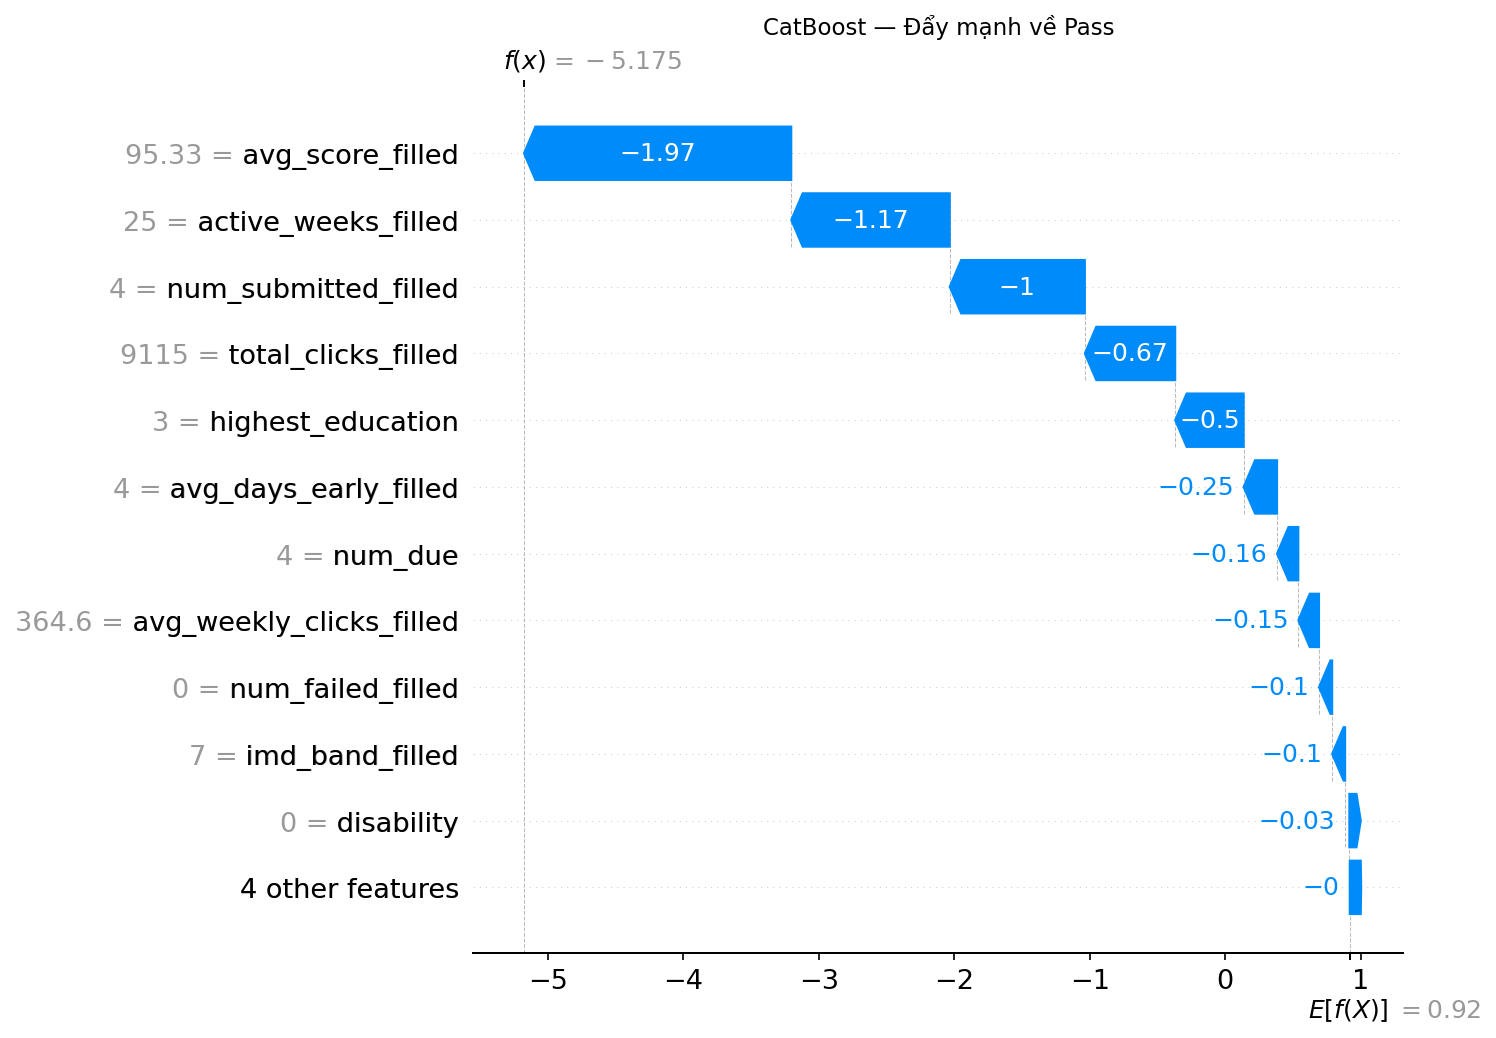
\includegraphics[width=\textwidth]{waterfall_pass.png}
    \caption{Trường hợp đẩy mạnh về Pass}
  \end{subfigure}
  \caption{Diễn giải cục bộ (waterfall) cho hai sinh viên đại diện.}
  \label{fig:waterfall}
\end{figure}

\begin{itemize}[leftmargin=*]
  \item \textbf{Trường hợp At-risk:} sinh viên chưa nộp bài nào
        (\code{num\_submitted\_filled} $= 0$, kéo theo \code{avg\_score\_filled}
        $= -1$ --- giá trị đánh dấu chưa có điểm) trong khi đã có 9 bài đến hạn
        (\code{num\_due} $= 9$). Hai yếu tố này đóng góp lần lượt $+2.60$ và
        $+3.01$ vào điểm số dự báo; cộng thêm số tuần hoạt động thấp
        (\code{active\_weeks\_filled} $= 6$, đóng góp $+1.24$), tổng điểm bị
        đẩy lên $8.84$ --- rất cao so với giá trị nền $0.92$, tương ứng xác
        suất At-risk gần như tuyệt đối.
  \item \textbf{Trường hợp Pass:} sinh viên có điểm trung bình cao
        (\code{avg\_score\_filled} $= 95.33$, kéo điểm số giảm $1.97$) và số
        tuần hoạt động nhiều (\code{active\_weeks\_filled} $= 25$, giảm
        $1.17$), cộng thêm lượt truy cập rất lớn
        (\code{total\_clicks\_filled} $= 9\,115$, giảm $0.67$) --- tổng hợp
        lại cho điểm số rất thấp ($-5.18$), tương ứng xác suất Pass gần như
        tuyệt đối.
\end{itemize}

Hai ví dụ trên cho thấy mô hình đưa ra quyết định dựa trên những tín hiệu phù
hợp với trực giác sư phạm: mức độ hoàn thành bài tập và điểm số tích luỹ là
yếu tố quyết định, đúng như đã được xác nhận qua phân tích độ quan trọng đặc
trưng ở quy mô toàn cục.

\section{Kết luận}

Từ toàn bộ quá trình xây dựng và so sánh mô hình, có thể rút ra các kết luận
chính sau:

\begin{itemize}[leftmargin=*]
  \item Việc gộp nhãn Fail và Withdrawn thành nhóm At-risk và giới hạn dữ liệu
        về mốc dự đoán 150 ngày đưa bài toán về dạng phân loại nhị phân, mất
        cân bằng nhãn ở mức vừa phải (At-risk chiếm khoảng 36\%) --- được
        xử lý hiệu quả bằng cách kết hợp SMOTE và trọng số lớp, đồng thời tinh
        chỉnh cả hai kỹ thuật này cùng với siêu tham số của từng mô hình thông
        qua Optuna.
  \item Trong số bốn thuật toán thử nghiệm, \textbf{CatBoost} đạt F1 At-risk
        cao nhất trên bộ đặc trưng đầy đủ (0.7849), đồng thời dẫn đầu cả về
        accuracy và precision; LightGBM bám sát ngay phía sau và giữ ROC-AUC
        cao nhất. Hai mô hình boosting này vượt trội hơn Logistic Regression
        một cách nhất quán trên mọi bộ đặc trưng, dù khoảng cách với Random
        Forest là không lớn.
  \item Hiệu suất mô hình \textbf{ổn định cao} khi giảm số lượng đặc trưng từ
        15 xuống chỉ còn 5 --- thậm chí CatBoost trên bộ Top-10 đạt F1
        At-risk cao nhất toàn thực nghiệm (0.7875). Kết quả này gợi ý một bộ
        \textbf{5 đặc trưng} (\code{num\_submitted\_filled},
        \code{avg\_score\_filled}, \code{num\_due}, \code{active\_weeks\_filled},
        \code{total\_clicks\_filled}) --- toàn bộ đều là đặc trưng hành vi học
        tập, không yêu cầu thông tin nhân khẩu học --- là đủ để xây dựng một hệ
        thống cảnh báo sớm gọn nhẹ, dễ triển khai và duy trì.
  \item Phân tích SHAP xác nhận các dự báo của mô hình dựa trên những tín hiệu
        phù hợp với trực giác sư phạm --- mức độ hoàn thành bài tập, điểm số
        tích luỹ và khối lượng công việc còn tồn đọng --- và các diễn giải này
        giữ nguyên tính nhất quán qua cả ba bộ đặc trưng.
\end{itemize}

\textbf{Hạn chế và hướng phát triển.} Nghiên cứu hiện chỉ đánh giá tại một mốc
thời gian duy nhất --- 150 ngày; một hướng mở rộng tự nhiên là huấn luyện và so
sánh mô hình tại \textbf{nhiều mốc dự đoán} khác nhau để xác định thời điểm
cảnh báo sớm nhất mà mô hình vẫn đạt độ tin cậy chấp nhận được, đồng thời theo
dõi cách các dự báo về cùng một sinh viên thay đổi theo thời gian. Bên cạnh
đó, việc \textbf{hiệu chỉnh ngưỡng phân loại} theo chi phí thực tế của việc bỏ
sót so với cảnh báo nhầm, cũng như thử nghiệm mô hình trên dữ liệu của các cơ
sở đào tạo khác, là những bước cần thiết trước khi đưa hệ thống vào vận hành
thực tế.

\end{document}
